% =============================================================================
%  Breadcrumbs
%  Blockchain Olympiad submission, Team CookieMonsters, United International
%  University.
%
%  HOW TO COMPILE
%    Upload main.tex and ref.bib to Overleaf. Set the compiler to pdfLaTeX.
%    Overleaf runs BibTeX automatically. Nothing else is needed: every figure
%    is drawn in TikZ inside this file, so there are no image files to upload.
%
%  >>> EDIT THE TEAM BLOCK BELOW BEFORE SUBMITTING <<<
% =============================================================================
\documentclass[11pt,a4paper]{article}

% ---- team details: replace the bracketed placeholders -----------------------
\newcommand{\TeamName}{CookieMonsters}
\newcommand{\TeamInstitution}{United International University, Dhaka, Bangladesh}
\newcommand{\TeamMembers}{Ahbab, Ruhi, Rohan, Ishmam, Adnan}
\newcommand{\TeamCategory}{Undergraduate}
\newcommand{\TeamContact}{mkhan223869@bscse.uiu.ac.bd}
% -----------------------------------------------------------------------------

\usepackage[T1]{fontenc}
\usepackage[utf8]{inputenc}
\usepackage{lmodern}
\usepackage[a4paper,margin=2.4cm]{geometry}
\usepackage{amsmath,amssymb}
\usepackage{graphicx}
\usepackage{xcolor}
\usepackage{booktabs}
\usepackage{tabularx}
\usepackage{array}
\usepackage{longtable}
\usepackage{caption}
\usepackage{enumitem}
\usepackage{titlesec}
\usepackage{fancyhdr}
\usepackage{tikz}
\usepackage{pgfplots}
\usepackage{algorithm}
\usepackage{algpseudocode}
\usepackage[numbers,sort&compress]{natbib}
\usepackage{hyperref}

\usetikzlibrary{positioning,shapes.geometric,arrows.meta,calc,fit,backgrounds}
\pgfplotsset{compat=1.18}

% ---- measured numbers ------------------------------------------------------
% Every figure in this report that came from running the system is pulled from
% results.tex, which is generated by the benchmarks in model/bench/ and is not
% edited by hand. A number that has not been measured renders as a bold ?? on the
% page rather than quietly appearing as something plausible.
%
% Regenerate with:  python -m model.bench.to_latex
\IfFileExists{results.tex}{% =============================================================================
%  results.tex — GENERATED. Do not edit.
%
%  Regenerate with:  python -m model.bench.to_latex   (from "Breadcrumbs Project")
%
%  Every macro below was produced by a benchmark in model/bench/. The paper refers
%  to them through \num{Name}, which prints the measurement if it exists and a
%  bold ?? if it does not — so an unmeasured number is visible on the page rather
%  than quietly absent.
% =============================================================================

\providecommand{\num}[1]{%
  \ifcsname res#1\endcsname\csname res#1\endcsname\else\textbf{??}\fi}
\providecommand{\numunit}[2]{%
  \ifcsname res#1\endcsname\csname res#1\endcsname\,#2\else\textbf{??}\fi}
\providecommand{\rows}[1]{%
  \ifcsname rows#1\endcsname\csname rows#1\endcsname\else
  \multicolumn{1}{l}{\textbf{?? not measured}}\\\fi}


% ---- accumulator.json: RSA accumulator costs and savings, 3072-bit modulus
\expandafter\def\csname resAccumulatorAccumulatorStateBytes\endcsname{384}
\expandafter\def\csname resAccumulatorAggregateBatchingSpeedup\endcsname{405}
\expandafter\def\csname resAccumulatorAggregateProvedMs\endcsname{8.99}
\expandafter\def\csname resAccumulatorAggregateRecords\endcsname{500}
\expandafter\def\csname resAccumulatorAggregateUnprovedMs\endcsname{3\,645}
\expandafter\def\csname resAccumulatorBatchAddMsPerRecord\endcsname{17.5}
\expandafter\def\csname resAccumulatorBatchAddRecords\endcsname{500}
\expandafter\def\csname resAccumulatorEpochExponentBits\endcsname{127\,789}
\expandafter\def\csname resAccumulatorEpochProofMs\endcsname{9.05}
\expandafter\def\csname resAccumulatorEpochProofSpeedup\endcsname{403}
\expandafter\def\csname resAccumulatorEpochRecomputeMs\endcsname{3\,646}
\expandafter\def\csname resAccumulatorEpochRecords\endcsname{500}
\expandafter\def\csname resAccumulatorHashToPrimeSpeedup\endcsname{2.20}
\expandafter\def\csname resAccumulatorMerkleProofsMs\endcsname{4.87}
\expandafter\def\csname resAccumulatorModulusBits\endcsname{3\,072}
\expandafter\def\csname resAccumulatorModulusGenerationSeconds\endcsname{2.10}
\expandafter\def\csname resAccumulatorSingleWitnessMs\endcsname{9.71}
\expandafter\def\csname resAccumulatorVerifierStateRootsBytes\endcsname{16\,000}
\expandafter\def\csname resAccumulatorHashToPrimeSearchMs\endcsname{3.55}
\expandafter\def\csname resAccumulatorHashToPrimeVerifyWithNonceMs\endcsname{1.61}
\expandafter\def\csname resAccumulatorAccumulatorAddOneRecordMs\endcsname{10.3}
\expandafter\def\csname resAccumulatorIssueTwoZeroWitnessesOneAtATimeMs\endcsname{2\,738}
\expandafter\def\csname resAccumulatorIssueTwoZeroWitnessesRootFactorMs\endcsname{647}
\expandafter\def\csname resAccumulatorIssueFourZeroWitnessesOneAtATimeMs\endcsname{11\,341}
\expandafter\def\csname resAccumulatorIssueFourZeroWitnessesRootFactorMs\endcsname{1\,604}
\expandafter\def\csname resAccumulatorIssueEightZeroWitnessesOneAtATimeMs\endcsname{45\,934}
\expandafter\def\csname resAccumulatorIssueEightZeroWitnessesRootFactorMs\endcsname{3\,763}
\expandafter\def\csname resAccumulatorVerifyFiveZeroRecordsAggregateWitnessWithBatchingProofMs\endcsname{9.09}
\expandafter\def\csname resAccumulatorVerifyFiveZeroRecordsAggregateWitnessNoBatchingProofMs\endcsname{375}
\expandafter\def\csname resAccumulatorVerifyFiveZeroRecordsFiveZeroBlockInclusionProofsMs\endcsname{0.413}
\expandafter\def\csname resAccumulatorVerifyOneZeroZeroRecordsAggregateWitnessWithBatchingProofMs\endcsname{10.2}
\expandafter\def\csname resAccumulatorVerifyOneZeroZeroRecordsAggregateWitnessNoBatchingProofMs\endcsname{763}
\expandafter\def\csname resAccumulatorVerifyOneZeroZeroRecordsOneZeroZeroBlockInclusionProofsMs\endcsname{0.930}
\expandafter\def\csname resAccumulatorVerifyTwoFiveZeroRecordsAggregateWitnessWithBatchingProofMs\endcsname{9.36}
\expandafter\def\csname resAccumulatorVerifyTwoFiveZeroRecordsAggregateWitnessNoBatchingProofMs\endcsname{1\,786}
\expandafter\def\csname resAccumulatorVerifyTwoFiveZeroRecordsTwoFiveZeroBlockInclusionProofsMs\endcsname{2.29}
\expandafter\def\csname resAccumulatorVerifyFiveZeroZeroRecordsAggregateWitnessWithBatchingProofMs\endcsname{8.99}
\expandafter\def\csname resAccumulatorVerifyFiveZeroZeroRecordsAggregateWitnessNoBatchingProofMs\endcsname{3\,645}
\expandafter\def\csname resAccumulatorVerifyFiveZeroZeroRecordsFiveZeroZeroBlockInclusionProofsMs\endcsname{4.87}
\expandafter\def\csname resAccumulatorVerifyOneMembershipWitnessMs\endcsname{9.71}
\expandafter\def\csname resAccumulatorVerifyAnEpochOfFiveZeroZeroRecordsByProofOfExponentiationMs\endcsname{9.05}
\expandafter\def\csname resAccumulatorVerifyTheSameEpochByRecomputingItMs\endcsname{3\,646}
% columns: direct_ms, n, with_proof_ms
\expandafter\def\csname rowsAccumulatorPoeCrossover\endcsname{%
7.53 & 1 & 8.96 \\
14.8 & 2 & 8.63 \\
36.9 & 5 & 8.53 \\
73.2 & 10 & 8.76 \\
182 & 25 & 8.63 \\
367 & 50 & 9.52 \\
729 & 100 & 9.08 \\}
% columns: eval_ms, iterations, ratio, verify_ms
\expandafter\def\csname rowsAccumulatorVdf\endcsname{%
50.8 & 1\,000 & 5.60 & 9.08 \\
537 & 10\,000 & 59.0 & 9.11 \\
2\,697 & 50\,000 & 294 & 9.17 \\
10\,950 & 200\,000 & 1\,132 & 9.68 \\}
% columns: aggregate_ms, aggregate_proof_bytes, aggregate_unproved_ms, merkle_ms, merkle_proof_bytes, n, verifier_state_bytes_accumulator, verifier_state_bytes_roots
\expandafter\def\csname rowsAccumulatorVerification\endcsname{%
9.09 & 1\,984 & 375 & 0.413 & 17\,600 & 50 & 384 & 1\,600 \\
10.2 & 3\,584 & 763 & 0.930 & 35\,200 & 100 & 384 & 3\,200 \\
9.36 & 8\,384 & 1\,786 & 2.29 & 88\,000 & 250 & 384 & 8\,000 \\
8.99 & 16\,384 & 3\,645 & 4.87 & 192\,000 & 500 & 384 & 16\,000 \\}
% columns: n, naive_ms, rootfactor_ms, speedup
\expandafter\def\csname rowsAccumulatorWitnessIssuance\endcsname{%
20 & 2\,738 & 647 & 4.23 \\
40 & 11\,341 & 1\,604 & 7.07 \\
80 & 45\,934 & 3\,763 & 12.2 \\}
\expandafter\def\csname resAccumulatorMachine\endcsname{macOS-26.6.1-arm64-arm-64bit}

% ---- identity.json: RSA-3072 identity and endorsement costs against the Ed25519 baseline
\expandafter\def\csname resIdentityCertificateCacheSpeedup\endcsname{18.5}
\expandafter\def\csname resIdentityEndorsementsAttached\endcsname{5}
\expandafter\def\csname resIdentityRsaSignSlowdown\endcsname{25.0}
\expandafter\def\csname resIdentityRsaSignatureGrowth\endcsname{6.00}
\expandafter\def\csname resIdentityRsaVerifySpeedup\endcsname{3.90}
\expandafter\def\csname resIdentitySignaturesAvoidedPerTransaction\endcsname{2}
\expandafter\def\csname resIdentitySignaturesVerifiedUnderPolicy\endcsname{3}
\expandafter\def\csname resIdentityEdTwoFiveFiveOneNineShaTwoFiveSixVOneGenerateAKeyMs\endcsname{0.083}
\expandafter\def\csname resIdentityEdTwoFiveFiveOneNineShaTwoFiveSixVOneSignATransactionMs\endcsname{0.083}
\expandafter\def\csname resIdentityEdTwoFiveFiveOneNineShaTwoFiveSixVOneVerifyASignatureMs\endcsname{0.187}
\expandafter\def\csname resIdentityRsaThreeZeroSevenTwoPssShaTwoFiveSixVOneGenerateAKeyMs\endcsname{111}
\expandafter\def\csname resIdentityRsaThreeZeroSevenTwoPssShaTwoFiveSixVOneSignATransactionMs\endcsname{2.08}
\expandafter\def\csname resIdentityRsaThreeZeroSevenTwoPssShaTwoFiveSixVOneVerifyASignatureMs\endcsname{0.048}
\expandafter\def\csname resIdentityResolveACertificateColdPerCallMs\endcsname{0.140}
\expandafter\def\csname resIdentityResolveACertificateCachedMs\endcsname{0.008}
\expandafter\def\csname resIdentityVerifyOneEndorsementEndToEndMs\endcsname{0.059}
% columns: certificate_bytes, disallowed_after, keygen_ms, public_key_bytes, sign_ms, signature_bytes, suite, verify_ms
\expandafter\def\csname rowsIdentitySuites\endcsname{%
558 & 2035-12-31 & 0.083 & 44 & 0.083 & 64 & ed25519-sha256-v1 & 0.187 \\
1\,529 & 2035-12-31 & 111 & 422 & 2.08 & 384 & rsa3072-pss-sha256-v1 & 0.048 \\}
\expandafter\def\csname resIdentityMachine\endcsname{macOS-26.6.1-arm64-arm-64bit}

% ---- ledger.json: Ledger write costs and epoch batching over 150 documents
\expandafter\def\csname resLedgerAssumedDocumentsPerFactoryMonth\endcsname{400}
\expandafter\def\csname resLedgerBlocksWritten\endcsname{152}
\expandafter\def\csname resLedgerCertificateCacheHits\endcsname{402}
\expandafter\def\csname resLedgerCertificateCacheMisses\endcsname{2}
\expandafter\def\csname resLedgerCertificateHitRate\endcsname{99.5}
\expandafter\def\csname resLedgerChainBytes\endcsname{1\,016\,492}
\expandafter\def\csname resLedgerChainBytesPerDocument\endcsname{6\,777}
\expandafter\def\csname resLedgerChainBytesPerFactoryYearKb\endcsname{31\,765}
\expandafter\def\csname resLedgerCommitMsPerDocument\endcsname{5.34}
\expandafter\def\csname resLedgerCommitTransactions\endcsname{152}
\expandafter\def\csname resLedgerDocuments\endcsname{150}
\expandafter\def\csname resLedgerDocumentsPerSecond\endcsname{187}
\expandafter\def\csname resLedgerEndorsementBytes\endcsname{2\,472}
\expandafter\def\csname resLedgerEpochBytes\endcsname{80\,579}
\expandafter\def\csname resLedgerEpochBytesPerDocument\endcsname{537}
\expandafter\def\csname resLedgerEpochMsPerDocument\endcsname{13.0}
\expandafter\def\csname resLedgerEpochSeconds\endcsname{1.95}
\expandafter\def\csname resLedgerEpochTransactions\endcsname{1}
\expandafter\def\csname resLedgerEpochWritesPerFactoryYear\endcsname{12}
\expandafter\def\csname resLedgerStorageReductionFactor\endcsname{12.6}
\expandafter\def\csname resLedgerTransactionBytes\endcsname{6\,367}
\expandafter\def\csname resLedgerWriteReduction\endcsname{150}
\expandafter\def\csname resLedgerValidateATransactionSEndorsementsMs\endcsname{0.135}
\expandafter\def\csname resLedgerMachine\endcsname{macOS-26.6.1-arm64-arm-64bit}

}{%
  \providecommand{\num}[1]{\textbf{??}}%
  \providecommand{\numunit}[2]{\textbf{??}}%
  \providecommand{\rows}[1]{\multicolumn{1}{l}{\textbf{?? not measured}}\\}}

% ---- palette (colour-blind safe, prints correctly in greyscale) -------------
\definecolor{tcblue}{HTML}{2563EB}
\definecolor{tcorange}{HTML}{E8710A}
\definecolor{tcgreen}{HTML}{059669}
\definecolor{tcgrey}{HTML}{6B7280}
\definecolor{tctext}{HTML}{111827}
\definecolor{tcline}{HTML}{E5E7EB}
\definecolor{tcbg}{HTML}{F7F8FA}

\hypersetup{colorlinks=true,linkcolor=tcblue,citecolor=tcblue,urlcolor=tcblue,
            breaklinks=true}

\titleformat{\section}{\normalfont\Large\bfseries\sffamily\color{tctext}}{\thesection}{0.7em}{}
\titleformat{\subsection}{\normalfont\large\bfseries\sffamily\color{tctext}}{\thesubsection}{0.6em}{}
\captionsetup{font=small,labelfont={bf,sf}}
\setlength{\parskip}{0.35em}
\renewcommand{\arraystretch}{1.18}

\pagestyle{fancy}\fancyhf{}
\lhead{\small\sffamily Breadcrumbs}
\rhead{\small\sffamily Team \TeamName}
\cfoot{\small\thepage}
\renewcommand{\headrulewidth}{0.4pt}

\raggedbottom
\newcolumntype{Y}{>{\raggedright\arraybackslash}X}
\newcommand{\est}{\textsuperscript{\textdagger}}

% ---- the logo, drawn rather than imported ----------------------------------
% A trail of marks, each one larger and more definite than the last, ending in
% the verified record. Drawn rather than imported so the file stays standalone.
\newcommand{\bclogo}[1][1.0]{%
\begin{tikzpicture}[scale=#1,every node/.style={transform shape}]
  \node[regular polygon,regular polygon sides=6,draw=tcblue,line width=1.5pt,
        minimum size=2.35cm,rotate=90] (hex) at (0,0) {};
  \draw[tcgrey!45,line width=1.0pt,dash pattern=on 1pt off 2.6pt,line cap=round]
        (-0.53,-0.36) -- (0.53,0.36);
  \fill[tcgrey!55] (-0.53,-0.36) circle (0.085);
  \fill[tcgrey]    (-0.27,-0.17) circle (0.110);
  \fill[tcblue]    ( 0.00, 0.00) circle (0.135);
  \fill[tcorange]  ( 0.27, 0.17) circle (0.155);
  \fill[tcgreen]   ( 0.53, 0.36) circle (0.180);
\end{tikzpicture}}

\begin{document}

% =============================================================================
% TITLE PAGE
% =============================================================================
\begin{titlepage}
\centering
\vspace*{1.2cm}
\bclogo[1.5]

\vspace{0.9cm}
{\sffamily\bfseries\Huge Breadcrumbs\par}
\vspace{0.35cm}
{\sffamily\large\color{tcgrey} every record leaves a trail anyone can check\par}

\vspace{1.4cm}
{\sffamily\LARGE\bfseries A Permissioned Blockchain with Federated\\[0.2cm]
Continual Learning for Verifiable Company\\[0.2cm]
Records in the Garment Industry\par}

\vspace{1.0cm}
{\large Built for Bangladesh first, designed to travel\par}

\vfill
\begin{tabular}{r l}
\textbf{Team} & \TeamName \\
\textbf{Institution} & \TeamInstitution \\
\textbf{Members} & \TeamMembers \\
\textbf{Category} & \TeamCategory \\
\textbf{Contact} & \TeamContact \\
\textbf{Date} & 14 August 2026 \\
\end{tabular}

\vspace{1.0cm}
{\small\color{tcgrey} Submitted to the Blockchain Olympiad Bangladesh\par}
\vspace{0.8cm}
\end{titlepage}

% =============================================================================
\section*{Executive Summary}
\addcontentsline{toc}{section}{Executive Summary}

In the 2025-26 financial year Bangladesh exported 38.7 billion US dollars of
clothing, which was 81 percent of everything the country sold abroad. That was
down from 39.3 billion the year before \citep{bgmea2026export}. Every shipment
rests on paperwork: wage registers, safety inspection reports, chemical
inventories, certificates, and purchase orders. Buyers in Europe and North
America do not trust that paperwork on its own, so they send auditors instead.
Factories pay for audit after audit, and the documents behind them can still be
edited afterwards.

Breadcrumbs is a permissioned blockchain that makes a company's own internal
records provable without publishing them, together with a shared fraud detector
that the ledger governs. A factory keeps its files; only commitments go on the
chain; anyone with permission can check that a document is genuine and unchanged
without ever seeing its contents.

\textbf{The part we think is new is not that a record can be proved genuine.}
Notarisation services have done that for years, and we say so plainly in
Section~\ref{sec:priorart}. It is that a factory can be made to prove
\emph{nothing is missing}. Every provenance system on the market answers ``is
this document real''. None of them answers ``is this every document, and was
anything withheld'', which is the question that matters, because the fraud that
actually happens is not a forged register but a second set of books and a
decision about which one to show. Breadcrumbs closes a reporting period into a
\emph{seal}: the contract enumerates every record the ledger holds for that site,
type and period, refuses to close unless the declaration matches, and commits a
count and a root. A factory that later discloses four of five sealed registers is
caught by arithmetic rather than by trust, and the four it did disclose all
verify perfectly.

Three further mechanisms sit around that one, and all four share a single
mathematical object: an RSA group of unknown order. It accumulates the entire
record set into one number, so a buyer verifying a year of payroll holds
\numunit{AccumulatorAccumulatorStateBytes}{bytes} of state rather than a copy of
every commitment. It produces \emph{non-membership} proofs, so ``no such
certificate was ever committed'' becomes cryptographic evidence rather than a
filing failure. It carries a batching proof that verifies an entire epoch in
\numunit{AccumulatorEpochProofMs}{ms}
against \numunit{AccumulatorEpochRecomputeMs}{ms} to recompute
it, a \num{AccumulatorEpochProofSpeedup}-fold reduction that does not grow with
the number of records. And it runs a verifiable delay function, so a colluding
majority cannot manufacture months of history over a weekend.

The fourth mechanism addresses the limitation every system of this kind concedes
and none solves: a ledger makes a record unchangeable but says nothing about
whether it was true when written. Each record is counter-signed by a second
organisation that is \emph{assigned rather than chosen}, from a seed no single
member controls, and that loses several times what honest attestation earns if
the record is later found false. This does not make records true. It converts
unilateral falsification into two-party collusion that is recorded and
attributable, and we state it exactly that way throughout.

Governing the learning plane is the Continuity Gate, which was specified but not
built when this report was first written and is now implemented and tested. A new
model version is promoted only if a threshold of independent organisations have
evaluated it against benchmarks whose hashes were committed before the round, and
only if it has not lost more than an agreed tolerance on any earlier task.

The system runs. It is \num{LedgerBlocksWritten} blocks and
\num{LedgerDocuments} documents in the measurements reported here, at
\numunit{LedgerDocumentsPerSecond}{committed documents per second}, and it passes
273 tests, 27 of which name a specific attack and try it. \textbf{Two of those
attacks succeed} and a third is bounded rather than prevented, and
Section~\ref{sec:security} reports all three: a colluding assigned witness is not
stopped, whoever holds the factorisation of the accumulator modulus can forge a
witness against the accumulator alone, and a model poisoned just inside the
gate's tolerance is promoted once, though repeating it is now caught by the
cumulative drift bound. We would rather present those than have them found.

The timing is deliberate. Bangladesh is scheduled to leave Least Developed
Country status on 24 November 2026, although a three-year deferral has been
requested and the decision rests with the United Nations General Assembly. Either
way, the country must increasingly compete on proof rather than price. European
due diligence duties on large buyers begin in 2029, and European obligations for
high-risk artificial intelligence, including automatic logging so a system's
behaviour can be traced, begin on 2 December 2027 after a deferral in July 2026.
Breadcrumbs is built for those dates, and it supports Sustainable Development
Goals 5, 8, 9, 12, 16 and 17.

% =============================================================================
\tableofcontents
\newpage

% =============================================================================
\section{How to read this report, and the words we use}

This report is written to be understood without a background in either
blockchain systems or machine learning. Every technical term is explained the
first time it appears. Table~\ref{tab:glossary} collects those explanations in
one place so you can look anything up while reading.

One term needs defining before anything else, because the whole proposal rests
on it. By \textbf{internal logical file} we mean any document a company creates
for its own operations and later has to justify to somebody outside. Examples
are a wage register, a fire drill log, a chemical stock sheet, a machine
maintenance record, a grievance report, a quality inspection sheet, and a
purchase order. These files are not public. They are not marketing material.
They are the actual evidence of how a company runs, and they are exactly what an
auditor, a buyer, or a regulator asks to see.

\begin{table}[htbp]
\centering
\caption{Terms used in this report, in plain language.}
\label{tab:glossary}
\small
\begin{tabularx}{\textwidth}{@{}l Y@{}}
\toprule
\textbf{Term} & \textbf{What it means here} \\
\midrule
Blockchain & A shared record book copied across several organisations. New
entries are chained to old ones using mathematics, so changing an old entry
would break every entry after it and everyone would notice. \\
Permissioned blockchain & A blockchain where every participant is a known,
approved organisation. There is no anonymous membership, no mining, and no
cryptocurrency. \\
Hyperledger Fabric & The specific permissioned blockchain software we use. It
is open source and widely deployed in industry \citep{androulaki2018fabric}. \\
Hash & A short fixed-length fingerprint calculated from a file. Change one
character in the file and the fingerprint changes completely. You cannot
recover the file from its fingerprint. \\
Merkle tree & A way of combining many hashes into one summary hash, arranged so
that you can prove one item was included without revealing the others
\citep{merkle1988signature}. \\
Smart contract & A program stored on the blockchain that all participants run
and agree on. In Hyperledger Fabric it is called chaincode. \\
Endorsement policy & The rule saying which organisations must approve a
transaction before it becomes valid, for example three signatures out of five. \\
Off-chain & Stored outside the blockchain, normally because the data is too
large or too confidential to share. \\
Federated learning & Training one shared model across many organisations where
the raw data never leaves its owner. Only model updates are exchanged
\citep{mcmahan2017fedavg}. \\
Model update & The set of numeric adjustments a model makes after seeing data.
It is not the data itself, but it is calculated from the data. \\
Continual learning & Teaching a model new things over time without retraining
it from the beginning \citep{parisi2019review}. \\
Catastrophic forgetting & The common failure where a model taught something new
becomes much worse at what it already knew \citep{kirkpatrick2017ewc}. \\
Fisher information & A measure of how important each internal setting of a model
was for a past task. One way to protect old knowledge. We tested it, measured it
as a net loss, and removed it (Section~\ref{sec:removed}). \\
Replay & Showing a model reminders of older material while it learns new
material, so it does not forget. \\
Differential privacy & Adding carefully sized random noise so that no single
record can be identified from what is published \citep{dwork2014dp}. \\
Secure aggregation & A method letting a server add up many parties' updates
while being unable to read any single one of them
\citep{bonawitz2017secagg}. \\
RMG & Ready-Made Garments, the clothing manufacturing and export sector. \\
BGMEA & Bangladesh Garment Manufacturers and Exporters Association, the main
industry body, with roughly 4{,}000 member factories
\citep{bgmea2026aware}. \\
DPP & Digital Product Passport, a European requirement for a digital record of
a product's materials and history \citep{eu2024espr}. \\
CSDDD & Corporate Sustainability Due Diligence Directive, the European law
obliging large companies to check their suppliers \citep{eu2024csddd}. \\
LDC & Least Developed Country, a United Nations classification that grants
Bangladesh reduced tariffs in several markets. \\
\bottomrule
\end{tabularx}
\end{table}

% =============================================================================
\section{The problem, seen from one factory}

Start in a knitwear factory in Gazipur with 2{,}000 workers. In a normal month
it produces a payroll register, an overtime log, a fire and electrical safety
checklist, a chemical purchase record, a machine servicing log, worker
grievance forms, and a set of shipping documents. All of it sits in
spreadsheets, in a local accounting package, and in paper folders.

Four things go wrong, and they compound.

\textbf{Nothing can be proved.} A spreadsheet can be edited today and given
yesterday's date. There is no way for the factory to demonstrate that its March
wage register is the same file it held in March. Honest factories suffer for
this as much as dishonest ones, because an honest record and a rewritten record
look identical. We should be careful about what we can cite here. We are not
aware of a published measurement of how often Bangladeshi factory records are
altered after the fact, and we do not assert a rate. The claim we make is about
capability, not frequency: nothing in the current system prevents it, and
nothing in the current system would reveal it.

What is documented is that the substitute works badly. Human Rights Watch
examined 40 social audit reports covering Bangladeshi factories and found
auditors reusing identical wording across different sites, and
freedom-of-association questions reported as having no findings or skipped
altogether \citep{hrw2023audits}. That is a finding about auditor effort, not
about tampered documents, and we cite it only for what it shows: audits are a
weak and expensive substitute for records that could simply be checked.

\textbf{The same work is done many times.} A factory supplying six buyers is
inspected against six overlapping standards, each requiring the same documents
assembled again by the same staff. Published starting prices from audit firms
run from roughly 700 to 800 US dollars per audit before the factory's own
preparation cost. That is a vendor list price, not a measured industry average.

\textbf{Useful data cannot be combined.} An algorithm could spot a forged
certificate, or a wage sheet whose arithmetic fails cross-checking. Building one
needs examples from many factories. No factory will send wage data to a
competitor, a buyer, or a platform. Buyer pricing is commercially sensitive.
Worker records are personal data, regulated in Bangladesh by the Personal Data
Protection Ordinance of 2025 and the Act that replaced it in 2026
\citep{bd2026pdpa}. So the data that would make detection possible stays locked
in thousands of separate offices.

\textbf{The rules will not stop moving.} Even a perfect detector built today
goes stale. New buyer codes arrive every year. European due diligence
obligations apply from 2029 \citep{eu2024csddd,ec2026csddd}, and the Digital
Product Passport for textiles follows the Ecodesign Regulation's indicative 2027
timeline \citep{eu2024espr}. Fraud methods evolve, and generative artificial
intelligence has made convincing forged documents cheap. A model must keep
learning, and a model that keeps learning tends to forget.

\subsection{Why this matters now}

Three deadlines converge, which is why we think this is a 2026 proposal rather
than a 2030 one.

Bangladesh is scheduled to graduate from Least Developed Country status on
24 November 2026, removing tariff preferences much of its export advantage
depends on. A three-year deferral has been requested and the decision rests with
the United Nations General Assembly \citep{un2026ldc}. Either way the direction
is fixed: as price advantage narrows, the surviving advantage is being easier
and safer to buy from.

Large European buyers will soon be legally answerable for their suppliers'
conduct, not merely embarrassed by it. We should be precise about how many
buyers that is, because the 2026 simplification package cut the scope sharply.
Due diligence duties now reach European companies with more than 5{,}000
employees and more than 1.5 billion euro of turnover, and non-European companies
with more than 1.5 billion euro of turnover inside the European Union
\citep{ec2026csddd}. That is far fewer buyers than the original directive
covered. It still includes the large retail groups that place the biggest orders
in Bangladesh, and those are exactly the buyers whose requirements the rest of
the market copies.

The third date moved recently, and we would rather correct it than repeat a
headline. The European Union's Artificial Intelligence Act was to apply to
high-risk systems from 2 August 2026. In July 2026 a further regulation deferred
that to 2 December 2027 for standalone high-risk systems and 2 August 2028 for
artificial intelligence embedded in regulated products \citep{eu2026aiomnibus}.
The Article 50 transparency duties were not deferred. So the regime is coming
later than planned, but it is coming. Article 12 requires high-risk systems to
log events automatically so their operation can be traced \citep{eu2024aiact}.
It requires logging; it does not require the log to be tamper-evident, and we do
not claim otherwise. Our claim is narrower: any system that must show which
model made which decision gets that record from Breadcrumbs as a by-product, in
a form no single participant can quietly revise.

% =============================================================================
\section{Why a blockchain, and where we deliberately do not use one}
\label{sec:whychain}

The most common failure in this field is using a blockchain where a database
would do. We applied the decision test of W\"{u}st and Gervais
\citep{wust2018blockchain}. A blockchain is justified when three conditions hold
together. Multiple parties must write to shared state, they do not fully trust
each other, and no single trusted authority is available or acceptable.

That test is satisfied here, and the parties are worth naming honestly. The
factory has reason to present its records favourably. The buyer has reason to
shift liability onto the supplier, and can dictate terms because it controls the
orders. Competing factories will not let a rival hold their data. The audit firm
is paid by the party it inspects. The regulator arrives after the fact. There is
no candidate for neutral custodian. If a factory ran the database, buyers would
not believe it. If a buyer ran it, no factory would join. If a vendor ran it,
both would depend on one company's commercial decisions.

A permissioned blockchain resolves this by making the record jointly held.
Hyperledger Fabric fits because participants are named organisations with issued
identities, confidentiality is enforced through separate channels and private
data collections, and there is no mining, no token, and no transaction fee
\citep{androulaki2018fabric}. Consensus is ordering-based rather than
competitive, so energy consumption is comparable to running ordinary database
servers. This matters: a judge is entitled to ask whether a blockchain proposal
is environmentally defensible, and for permissioned systems the honest answer is
that the mining energy problem does not arise.

We are equally clear about what does not belong on a ledger. Table~\ref{tab:onchain}
sets out the split. Documents, model weights, and personal data stay off-chain.
Blockchain systems are slow and expensive compared with databases for bulk
storage \citep{dinh2018untangling}, and putting personal data on an
append-only ledger would conflict with deletion rights under Bangladesh's data
protection law. The ledger holds commitments and decisions, nothing more.

\begin{table}[htbp]
\centering
\caption{What Breadcrumbs writes to the ledger, and what it deliberately keeps
off it. The right-hand column is the answer to ``why not just use a database''.}
\label{tab:onchain}
\small
\begin{tabularx}{\textwidth}{@{}l l Y@{}}
\toprule
\textbf{Item} & \textbf{Where} & \textbf{Reason} \\
\midrule
Document hash and Merkle root & On-chain & Small, and proves a file existed
unchanged at a time. A party who could edit this could rewrite history. \\
Document metadata (type, period, issuing site) & On-chain & Needed for
verification and search. Contains no personal or commercial detail. \\
Access grant and revocation & On-chain & A buyer must not be able to deny that
access was granted, and a factory must not be able to deny granting it. \\
Model version identifier and its parent & On-chain & Establishes which model
made a decision, which the AI Act requires to be traceable. \\
Prototype memory-bank hash & On-chain & Proves which memory the
model was consolidated against, so training can be re-checked. \\
Continuity Gate result and metrics & On-chain & The promotion decision must be
enforced by rule, not by whoever operates the server. \\
Contribution and reputation score & On-chain & Determines rewards and access;
a participant could otherwise be quietly downgraded. \\
\midrule
The document file itself & Off-chain & Too large, confidential, and must remain
deletable. \\
Worker names, wages, national ID numbers & Off-chain & Personal data. Never
written to an append-only store. \\
Model weights and gradients & Off-chain & Large, and updated far too often for
ledger economics. \\
Training records and features & Off-chain & The entire point of federated
learning is that these never move. \\
\bottomrule
\end{tabularx}
\end{table}

% =============================================================================
\section{What already exists, and the gap we are filling}
\label{sec:priorart}

This is not an empty field, and we would rather say so than be told so.

\textbf{On the research side}, federated learning is well established
\citep{mcmahan2017fedavg,kairouz2021advances}, as are its standard defences:
secure aggregation \citep{bonawitz2017secagg}, differential privacy
\citep{abadi2016dpsgd}, and robust averaging against dishonest participants
\citep{blanchard2017krum,yin2018byzantine}. Blockchains have been combined with
federated learning since BlockFL \citep{kim2020blockfl} and extended to
industrial settings \citep{lu2020blockchainfl,nguyen2021flblockchain}. Swarm
Learning demonstrated a blockchain-coordinated federation on real clinical data
in \emph{Nature} \citep{warnat2021swarm}. Continual learning has mature method
families: penalising changes to important weights \citep{kirkpatrick2017ewc},
replaying stored or generated examples \citep{rebuffi2017icarl,shin2017dgr}, and
constrained gradient updates \citep{lopezpaz2017gem}. Federated continual
learning is a named field, with FedWeIT an early landmark
\citep{yoon2021fedweit} and several recent surveys
\citep{hamedi2025fcl,wang2024fcledge,gholizade2026fcl}.

\textbf{On the commercial side}, the closest activity is in traceability rather
than internal records. TextileGenesis and TrusTrace track materials through
supply chains. The Aura Blockchain Consortium issues product passports for
luxury brands. Most relevant of all, BGMEA has already moved. It signed an
agreement with DigiProd Pass in May 2025 for a Digital Product Passport pilot
\citep{bgmea2025digiprod}. It signed another with the Dutch platform AWARE on
10 May 2026, covering blockchain-based passport readiness across its member
factories \citep{bgmea2026aware}.

We treat that as the strongest evidence in this report, and we are direct about
what it means for us. BGMEA signing two blockchain traceability agreements
proves the demand is real and the industry body is willing. It also means we
would be unwise to compete with them, so we do not. Those systems answer ``where
did this garment's cotton come from''. They record product and material flow.
They say nothing about whether the factory's own wage register is authentic, and
nothing about learning from documents. Breadcrumbs sits underneath a Digital
Product Passport and supplies the internal evidence that makes its claims worth
believing. A passport asserting that a factory paid legal wages is only as good
as the wage record behind it.

Table~\ref{tab:market} sets out the comparison. Note that we lose several
columns outright. Notarisation services already make documents tamper-evident,
and LiFeChain already puts federated lifelong learning on a blockchain. The
columns nobody else fills are the last three.

\begingroup
\scriptsize
\setlength{\tabcolsep}{2.5pt}
\begin{longtable}{@{}>{\raggedright\arraybackslash}p{2.8cm}
  >{\centering\arraybackslash}p{1.1cm}
  >{\centering\arraybackslash}p{1.25cm}
  >{\centering\arraybackslash}p{1.1cm}
  >{\centering\arraybackslash}p{1.1cm}
  >{\centering\arraybackslash}p{1.25cm}
  >{\centering\arraybackslash}p{1.6cm}
  >{\centering\arraybackslash}p{1.0cm}
  >{\raggedright\arraybackslash}p{3.3cm}@{}}
\caption{Comparison with existing systems. ``Internal records'' means a
company's own operating documents rather than product or material flow.
``Absence'' means the system can prove a record was \emph{never} committed.
``Completeness'' means it can prove a disclosed set is the whole set for a period.
``Witness'' means an independent organisation counter-signs at capture. A dash
means the capability is absent, not merely weaker.}
\label{tab:market}\\
\toprule
\textbf{System} & \textbf{Ledger} & \textbf{Internal} & \textbf{Shared} &
\textbf{Gate on} & \textbf{Absence} & \textbf{Complete-} & \textbf{Wit-} &
\textbf{Primary purpose} \\
 & & \textbf{records} & \textbf{model} & \textbf{past tasks} & & \textbf{ness} & \textbf{ness} & \\
\midrule
\endfirsthead
\multicolumn{9}{@{}l}{\scriptsize\tablename~\thetable{} (continued)}\\
\toprule
\textbf{System} & \textbf{Ledger} & \textbf{Internal} & \textbf{Shared} &
\textbf{Gate on} & \textbf{Absence} & \textbf{Complete-} & \textbf{Wit-} &
\textbf{Primary purpose} \\
 & & \textbf{records} & \textbf{model} & \textbf{past tasks} & & \textbf{ness} & \textbf{ness} & \\
\midrule
\endhead
\bottomrule
\endfoot
TextileGenesis, TrusTrace & yes & -- & -- & -- & -- & -- & -- & Material and fibre traceability \\
AWARE, DigiProd Pass (BGMEA) & yes & -- & -- & -- & -- & -- & -- & Digital Product Passport readiness \\
Aura Consortium & yes & -- & -- & -- & -- & -- & -- & Luxury product authenticity \\
Sedex/SMETA, amfori BSCI & -- & partial & -- & -- & -- & -- & partial & Audit reports and sharing \\
IBM Food Trust & yes & -- & -- & -- & -- & -- & -- & Food supply provenance \\
Guardtime, OpenTimestamps, QLDB & partial & yes & -- & -- & -- & -- & -- & Document notarisation, tamper-evident logs \\
Certificate Transparency & yes & -- & -- & -- & partial & -- & yes & Public log of issued certificates \\
Accumulator ledger observers \citep{abebe2021observation} & yes & -- & -- & -- & yes & -- & -- & External verification of ledger state \\
Owkin, NVIDIA FLARE, Flower & -- & -- & yes & -- & -- & -- & -- & Federated learning tooling \\
Swarm Learning \citep{warnat2021swarm} & yes & -- & yes & -- & -- & -- & -- & Decentralised clinical training \\
BAFFLE, VFChain, committee designs & yes & -- & yes & -- & -- & -- & -- & On-chain validation of single updates \\
IBM US 11,157,833 \citep{calmon2021patent} & yes & -- & yes & -- & -- & -- & -- & On-chain threshold check on a withheld test set \\
LiFeChain \citep{chen2025lifechain} & yes & -- & yes & -- & -- & -- & -- & Blockchain for federated lifelong learning \\
FedWeIT \citep{yoon2021fedweit} & -- & -- & yes & -- & -- & -- & -- & Federated continual learning method \\
Model registries, MLOps gates & -- & -- & -- & partial & -- & -- & -- & Accuracy gate, single-owner, not pre-committed \\
\midrule
\textbf{Breadcrumbs} & yes & yes & yes & yes & yes & yes & yes & Verifiable internal records, provably complete \\
\bottomrule
\end{longtable}
\endgroup

\subsection{The closest prior art, and exactly what is different}

Several systems already move parts of federated learning onto a blockchain and
let a contract decide whether an update is acceptable. BAFFLE removes the
central aggregator and coordinates rounds through contracts
\citep{ramanan2020baffle}. VFChain records training so the process can be
audited afterwards \citep{peng2022vfchain}. Committee designs have a rotating
group of nodes score each update and vote \citep{li2021committee}. Closer still,
IBM holds a granted patent in which a withheld test set is held on a ledger, a
submitted model is run against it, and the result is checked against a
performance threshold \citep{calmon2021patent}. LiFeChain is a blockchain built
for federated \emph{lifelong} learning \citep{chen2025lifechain}. And outside
blockchains entirely, refusing to promote a model that has regressed is ordinary
practice in model registries.

None of the cryptography here is ours either, and it would be worse than useless
to imply otherwise. RSA accumulators go back to Benaloh and de Mare
\citep{benaloh1994accumulator} and Camenisch and Lysyanskaya
\citep{camenisch2002accumulator}; non-membership witnesses to Li, Li and Xue
\citep{li2007nonmembership}; the batching, aggregation and proof-of-exponentiation
techniques we rely on to Boneh, B\"{u}nz and Fisch \citep{boneh2019batching};
verifiable delay functions to Boneh and colleagues \citep{boneh2018vdf} and the
succinct proof we use to Wesolowski \citep{wesolowski2020vdf}. Applying an
accumulator to a Fabric ledger has been done: Abebe and colleagues maintain a
dynamic RSA accumulator as a digest of Fabric state so external clients can verify
it without running a peer \citep{abebe2021observation}. Witness co-signing, where a
statement is not accepted until a diverse group has publicly observed it, is
Syta and colleagues' CoSi \citep{syta2016cosi}, and Certificate Transparency has
run a version of it at internet scale for a decade \citep{laurie2014ct}.

What we have not found anywhere is the combination of a \emph{sealed reporting
period} with an accumulator, so that a verifier can establish not merely that a
disclosed record is genuine but that the disclosed set is the entire set, and
the pairing of that with an independent counter-signatory who is assigned by a
seed no participant controls and who is penalised when the record is later found
false. Stated as narrowly as we can defend it, the contribution is that
\textbf{withholding becomes an arithmetic contradiction rather than an invisible
act}, in a setting where the parties have concrete reasons to distrust each other.
The individual primitives are all borrowed, and we have named who from.

So neither on-chain model validation nor blocking a harmful update is new, and
we claim neither. What those systems check is whether a model is good enough
\emph{now}, against one threshold or one withheld set. Our gate asks whether a
candidate has become worse at each of several \emph{earlier} tasks, each
measured against its own frozen benchmark whose hash was committed before the
round, in a consortium where no participant can override the outcome. A
committee voting on update quality cannot detect forgetting, because forgetting
does not make an update look bad. It makes it look excellent, on the only data
the committee is looking at.

Stated as narrowly as we can defend it: our contribution is a promotion rule
that is backward-looking over pre-committed per-task benchmarks and enforced
collectively rather than by whoever runs the server. We have not found that
combination elsewhere, we do not claim to have invented on-chain model gating,
and the IBM patent is something any team building this would need advice on.

% =============================================================================
\section{System design}

Breadcrumbs has three planes. Figure~\ref{fig:arch} shows how they fit together.

\begin{figure}[htbp]
\centering
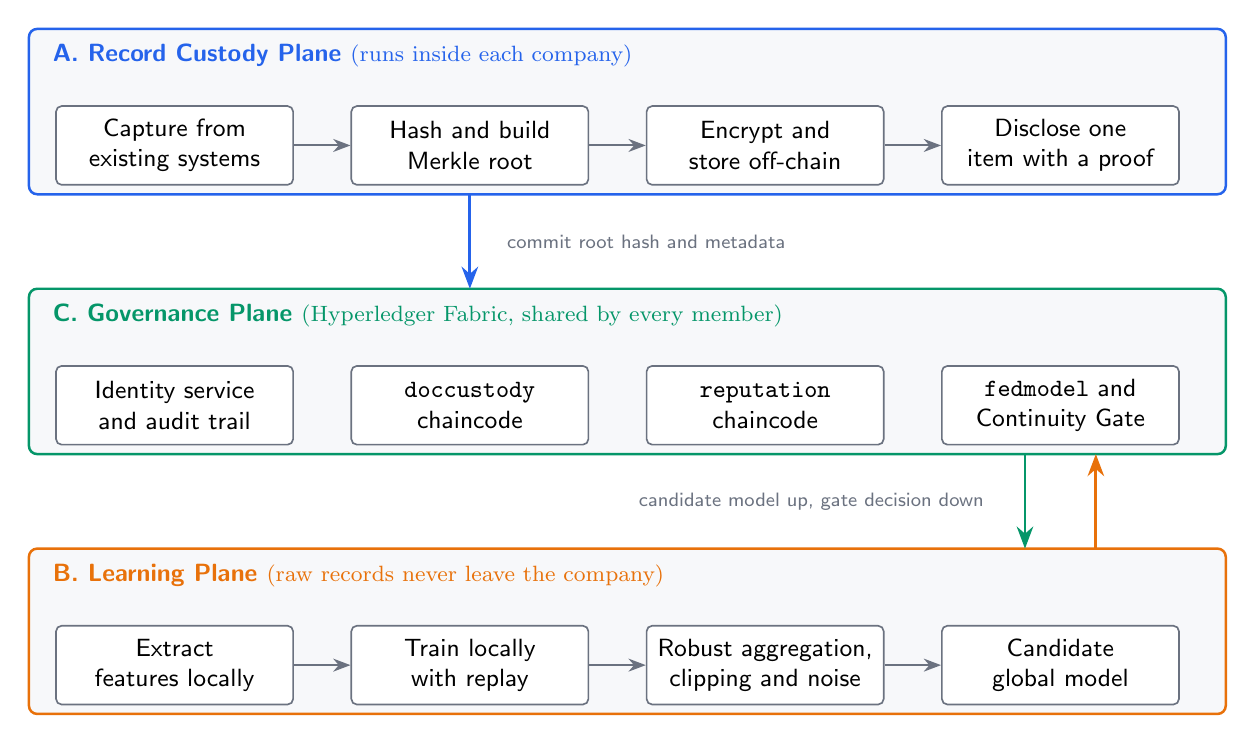
\begin{tikzpicture}[
  font=\sffamily\small,
  box/.style={rounded corners=2pt,draw=tcgrey,fill=white,line width=0.6pt,
              minimum height=1.0cm,text width=2.8cm,align=center,inner sep=3pt},
  band/.style={rounded corners=3pt,line width=0.9pt},
  lbl/.style={font=\sffamily\bfseries\small,align=left},
  ar/.style={-{Stealth[length=2.8mm]},line width=1.0pt},
  flow/.style={-{Stealth[length=2.2mm]},line width=0.7pt,tcgrey},
  tag/.style={font=\sffamily\scriptsize,text=tcgrey}]

% ---- Plane A: record custody (top) ----
\fill[tcbg,band,draw=tcblue] (0,7.0) rectangle (15.2,9.1);
\node[lbl,anchor=north west,text=tcblue] at (0.18,9.03)
  {A. Record Custody Plane \normalfont\footnotesize(runs inside each company)};
\node[box] (a1) at (1.85,7.62) {Capture from existing systems};
\node[box] (a2) at (5.60,7.62) {Hash and build Merkle root};
\node[box] (a3) at (9.35,7.62) {Encrypt and store off-chain};
\node[box] (a4) at (13.10,7.62) {Disclose one item with a proof};
\draw[flow] (a1) -- (a2); \draw[flow] (a2) -- (a3); \draw[flow] (a3) -- (a4);

% ---- Plane C: governance (middle, because it mediates the other two) ----
\fill[tcbg,band,draw=tcgreen] (0,3.7) rectangle (15.2,5.8);
\node[lbl,anchor=north west,text=tcgreen] at (0.18,5.73)
  {C. Governance Plane \normalfont\footnotesize(Hyperledger Fabric, shared by every member)};
\node[box] (c1) at (1.85,4.32) {Identity service and audit trail};
\node[box] (c2) at (5.60,4.32) {\texttt{doccustody} chaincode};
\node[box] (c3) at (9.35,4.32) {\texttt{reputation} chaincode};
\node[box] (c4) at (13.10,4.32) {\texttt{fedmodel} and Continuity Gate};

% ---- Plane B: learning (bottom) ----
\fill[tcbg,band,draw=tcorange] (0,0.4) rectangle (15.2,2.5);
\node[lbl,anchor=north west,text=tcorange] at (0.18,2.43)
  {B. Learning Plane \normalfont\footnotesize(raw records never leave the company)};
\node[box] (b1) at (1.85,1.02) {Extract\\features locally};
\node[box] (b2) at (5.60,1.02) {Train locally with replay};
\node[box] (b3) at (9.35,1.02) {Robust aggregation, clipping and noise};
\node[box] (b4) at (13.10,1.02) {Candidate global model};
\draw[flow] (b1) -- (b2); \draw[flow] (b2) -- (b3); \draw[flow] (b3) -- (b4);

% ---- cross-plane couplings: short, vertical, in the gaps ----
\draw[ar,tcblue] (5.60,7.0) -- (5.60,5.8);
\node[tag,anchor=west] at (5.95,6.40) {commit root hash and metadata};

\draw[ar,tcorange] (13.55,2.5) -- (13.55,3.7);
\draw[ar,tcgreen]  (12.65,3.7) -- (12.65,2.5);
\node[tag,anchor=east] at (12.25,3.10) {candidate model up, gate decision down};
\end{tikzpicture}
\caption{The three planes of Breadcrumbs. Plane A makes a company's own documents
provable without publishing them. Plane B builds a shared detector without
moving data. Plane C, the permissioned ledger, sits between them: it holds the
document commitments from above and decides whether a new model version from
below is allowed to replace the current one. Schematic diagram.}
\label{fig:arch}
\end{figure}

\subsection{Plane A: making a document provable}

When a document is finalised, an agent inside the factory hashes it. Line-level
items, for example one worker's row in a wage register, are hashed individually
and combined into a Merkle tree. The root hash, document type, reporting period
and site identifier go to the ledger. The document itself is encrypted with the
factory's key and stored off-chain \citep{benet2014ipfs}.

The Merkle structure is what makes selective disclosure possible
\citep{merkle1988signature}. A factory can prove one specific line belongs to
the committed register by revealing that line and a short proof path, while
every other line stays hidden. An auditor investigating one worker's overtime
claim does not get the whole payroll. That is a real improvement on current
practice, where producing evidence means handing over the entire file.

Figure~\ref{fig:seq} traces a complete verification.

\begin{figure}[htbp]
\centering
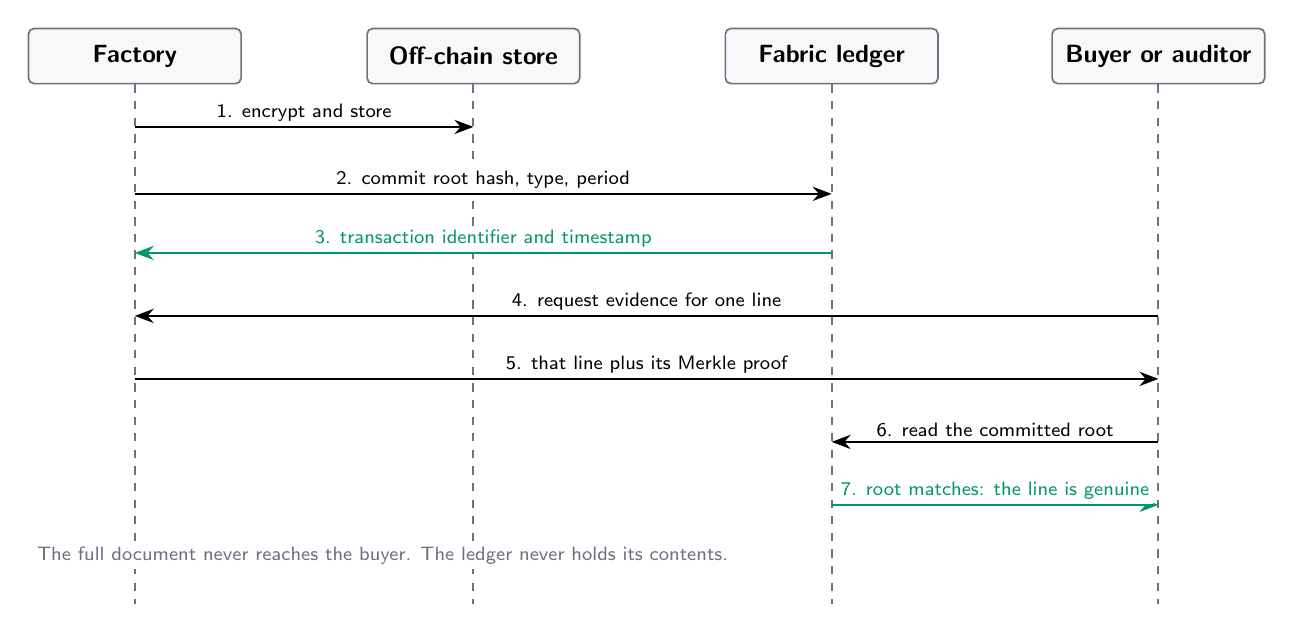
\begin{tikzpicture}[font=\sffamily\small,
  ll/.style={draw=tcgrey,line width=0.7pt,dashed},
  hd/.style={rounded corners=2pt,draw=tcgrey,fill=tcbg,line width=0.6pt,
             minimum height=0.7cm,minimum width=2.7cm,align=center,font=\sffamily\small\bfseries},
  msg/.style={-{Stealth[length=2.4mm]},line width=0.8pt},
  st/.style={font=\sffamily\scriptsize,align=center,fill=white,inner sep=1.5pt}]

\node[hd] (F) at (1.45,0)  {Factory};
\node[hd] (S) at (5.75,0)  {Off-chain store};
\node[hd] (L) at (10.3,0)  {Fabric ledger};
\node[hd] (B) at (14.45,0) {Buyer or auditor};
\foreach \n in {F,S,L,B} \draw[ll] (\n.south) -- ++(0,-6.6);

\draw[msg] (1.45,-0.9)  -- node[st,above]{1. encrypt and store} (5.75,-0.9);
\draw[msg] (1.45,-1.75) -- node[st,above]{2. commit root hash, type, period} (10.3,-1.75);
\draw[msg,tcgreen] (10.3,-2.5) -- node[st,above]{3. transaction identifier and timestamp} (1.45,-2.5);
\draw[msg] (14.45,-3.3) -- node[st,above]{4. request evidence for one line} (1.45,-3.3);
\draw[msg] (1.45,-4.1)  -- node[st,above]{5. that line plus its Merkle proof} (14.45,-4.1);
\draw[msg] (14.45,-4.9) -- node[st,above]{6. read the committed root} (10.3,-4.9);
\draw[msg,tcgreen] (10.3,-5.7) -- node[st,above]{7. root matches: the line is genuine} (14.45,-5.7);
\node[st,text=tcgrey,anchor=west] at (0.15,-6.35)
  {The full document never reaches the buyer. The ledger never holds its contents.};
\end{tikzpicture}
\caption{Verifying a single line of a wage register without disclosing the rest
of it. Steps 4 to 7 need no cooperation from the factory beyond serving the
proof. Schematic diagram; we have not built this, so we quote no timings.}
\label{fig:seq}
\end{figure}

\subsection{Plane B: learning without collecting data}
\label{sec:planeb}

Each factory extracts numeric features from its own documents. Some check
arithmetic: do stated totals match their components, are overtime hours
consistent. Some check form: does a certificate identifier match the issuing
body's format, do timestamps fall in a plausible order. Some check history: how
far a value sits from what this site normally reports. All are computed locally
and never leave the factory.

Training follows federated averaging \citep{mcmahan2017fedavg}, with FedProx-style
regularisation to cope with factories holding very different data
\citep{li2020fedprox}. Because model updates can leak information about the data
that produced them \citep{zhu2019dlg,geiping2020inverting,shokri2017membership},
we do not claim that federated learning is private by itself. Updates are
clipped and noise is added before they are sent \citep{abadi2016dpsgd}.

Here we have to declare a conflict rather than list three defences and hope
nobody checks. Secure aggregation hides individual updates and reveals only
their sum \citep{bonawitz2017secagg}. Coordinate-wise trimmed mean discards
extreme values, which requires ranking each participant's contribution
\citep{yin2018byzantine}. Contribution scoring requires attributing quality to
named participants. The second and third need to see what the first is designed
to hide. You cannot simply have all three.

Our choice for the first deployment is to run robust aggregation and
contribution scoring on updates that the aggregator can read, and to rely on
clipping, added noise, and locally engineered features for privacy rather than
on cryptographic hiding. That is a weaker privacy position than secure
aggregation and we state it plainly. Secure aggregation becomes possible later
through committee decryption or by ranking under multi-party computation, at
a cost in protocol complexity that a first pilot does not need. The alternative,
claiming all three at once, would not survive the first competent question.

\subsection{Plane C: the ledger as governor}

Three chaincodes run on Fabric. \texttt{doccustody} records document commitments
and access grants. \texttt{fedmodel} records every training round, its
contributors, the memory-bank hash, and the promotion decision.
\texttt{reputation} maintains a contribution score that weights aggregation and
controls model access. Two channels separate concerns: a document channel per
factory-buyer pair, so one buyer cannot see another's orders, and a model
channel shared by all members. Personal data appears on neither.

% =============================================================================
\section{What is new: one group, four jobs}
\label{sec:novel}

The architecture above is a sound combination of known parts. Hash-chained
blocks, Merkle commitments, X.509 membership and endorsement policies are
competent engineering, not contribution, and we do not present them as such.
What follows is what we believe is new.

Everything in this section rests on one object. RSA gives a \emph{group of
unknown order}: a set with multiplication where nobody can work out how many
elements it has. That single property does four separate jobs, and the fact that
it is one property rather than four unrelated features is the shape of the
contribution.

\begin{enumerate}[leftmargin=1.5em,itemsep=0.2em]
\item It accumulates the whole record set into one number, with a constant-size
      \textbf{membership witness} per record.
\item It produces \textbf{non-membership witnesses}, which is how absence becomes
      provable.
\item It carries a \textbf{proof of exponentiation}, which is how an epoch of any
      size is verified in constant time.
\item It runs a \textbf{verifiable delay function}, which is how elapsed time is
      bounded without trusting anybody's clock.
\end{enumerate}

Choosing RSA has a cost and we measure it rather than argue it away
(Section~\ref{sec:performance}): signing is
\num{IdentityRsaSignSlowdown} times slower than Ed25519 and signatures are
\num{IdentityRsaSignatureGrowth} times larger. One result went the other way and
is worth flagging because it is counter-intuitive: RSA \emph{verification} is
\num{IdentityRsaVerifySpeedup} times \emph{faster} than Ed25519, and a ledger
verifies far more often than it signs.

\subsection{Period seals, and proving that nothing is missing}
\label{sec:seals}

This is the mechanism we would defend hardest, and the one we would put in a
single sentence if given one: \textbf{existing systems prove a record is real;
this proves that nothing is missing.}

Consider what a notarisation service actually establishes. A factory hands a
buyer four payroll registers. Each one is genuine, each hash matches its
commitment, each Merkle proof verifies. Every system in Table~\ref{tab:market}
reports success. And the factory held back a fifth register, which is where the
problem was. Nothing was forged. Nothing was edited. The fraud was entirely in
the selection, and no amount of per-document integrity touches it.

A \emph{bucket} is one owner's records of one type, at one site, for one period.
Closing a bucket is a transaction:

\begin{itemize}[leftmargin=1.4em,itemsep=0.15em]
\item The contract enumerates every record the ledger holds for that bucket and
      \textbf{refuses to seal if the declared list omits any of them}. A seal a
      factory could compute over whatever subset it liked would prove only that
      it can do arithmetic.
\item It commits the count and a Merkle root over the sorted record identifiers.
\item Afterwards, committing into that bucket is refused. A record that genuinely
      arrives late goes through an \emph{amendment}, which keeps the previous
      count and root in a permanent history and demands a written reason.
\end{itemize}

A verifier then checks completeness with arithmetic and nothing else: recompute
the root over what you were given, compare the count. The factory withholding one
register produces a root that does not match and a count that is short by one,
and the four registers it did disclose still verify perfectly, which is
exactly the point, because that is the situation every existing system reports as
clean.

The amendment path deserves a note, because forbidding late records would make
the system unusable by honest factories and we would rather price a legitimate
action than ban it. An amendment costs reputation and is permanently visible, so
a factory whose amendment rate sits far above its peers has told the consortium
something whether it meant to or not.

\textbf{What this does not do.} It cannot make a factory commit a record it never
committed. A register kept entirely off the ledger leaves a seal that is
internally consistent and says nothing. Sealing defeats \emph{withholding at
disclosure}, which is a large and specific fraud, and it does not defeat
\emph{never recording}, which is the first-mile problem the next mechanism
narrows. Anyone presenting seals as a solution to fraud rather than to
withholding is overstating them, and we have tried not to.

\subsection{Attesting witnesses, assigned rather than chosen}
\label{sec:witness}

Section~\ref{sec:hardquestions} concedes the limitation every provenance system
shares: a signed record of a false statement is still a correct record of a lie.
This narrows it.

Each record is counter-signed at capture by a second organisation. Three details
decide whether that is a control or a formality, and all three are enforced by
the contract rather than by convention.

\textbf{The witness is assigned, not chosen.} A factory that picks its own
counter-signatory has bought an alibi. The assignment is computed from a hash of
a shared seed and the record's own identifier, so it is deterministic. Every
endorsing peer derives the same answer, which is what chaincode requires, and the
factory cannot influence it.

\textbf{The seed comes from commit--reveal.} Each member commits to the hash of a
share before anybody reveals theirs. A member choosing its share does not yet know
anyone else's, so the assignment is unpredictable to all of them unless every
single member colludes. Without the commit phase, whoever revealed last could try
values until the assignment suited them.

\textbf{The witness says what it actually did.} An attestation carries a check
code: format only, sample rows recomputed, totals read back from the source
system, or somebody physically present. These are different claims carrying
different weight, and a witness that signs the strongest one for a record later
found false has made a specific, attributable assertion rather than a gesture.

The consequence is what gives it force. Attesting honestly earns a small
reputation credit; attesting to a record later found false costs more than four
times that. Findings are filed by an auditor organisation, are permanent, and
name every organisation that vouched.

Witnessing everything would be right for a paper and wrong for a factory
producing four hundred documents a month, so high-stakes types, payroll and
safety, are always witnessed and the rest are sampled at a rate the consortium
sets, drawn from the same shared seed so a factory cannot know in advance which
of its routine records will be checked.

\textbf{What this does not do,} stated as plainly as we can: an assigned witness
willing to sign for a document it never examined is not stopped, and our test
suite contains a passing test that demonstrates exactly that. The claim we make
is narrow and we make it in these words: unilateral falsification becomes
two-party collusion that is recorded, attributable and penalised. It is not a
claim that records are true.

\subsection{The accumulator: constant-size state, constant-time verification}
\label{sec:accumulator}

Every record and every seal is mapped to a prime and folded into a single
accumulator value. A membership witness is that value with the record's prime
divided out; raising the witness to the prime returns the accumulator. Forging one
means computing a root nobody can compute without the modulus's factorisation,
which is the strong RSA assumption.

Three things follow that a Merkle tree cannot provide at any price.

\textbf{Absence becomes provable.} A buyer shown a compliance certificate can
obtain a non-membership witness: cryptographic proof that no such record was ever
committed. ``We hold no record of that'' stops being a filing failure and becomes
evidence.

\textbf{Verification stops depending on ledger size.} A verifier holds
\numunit{AccumulatorAccumulatorStateBytes}{bytes}, one group element, rather
than a copy of every commitment it might need to check against. That is what makes
it realistic for a European buyer to verify a Bangladeshi factory's records
without running a peer.

\textbf{Many records verify as cheaply as one.} Witnesses aggregate, and the
aggregate carries a batching proof. Measured, verification of an aggregate is
essentially flat in the number of records it covers, where the same check without
the proof grows linearly and becomes slower than simply checking every Merkle
proof separately. We report both, because the naive construction losing to Merkle
is a real result and hiding it would make the table dishonest.

Batching also changes the ledger's cost model. Committing one transaction per
document is what makes people abandon blockchains for record-keeping. Folding an
epoch into a single accumulator update takes \num{LedgerDocuments} documents from
\num{LedgerCommitTransactions} ledger writes to
\num{LedgerEpochTransactions}, and per-document chain growth falls by a factor of
\num{LedgerStorageReductionFactor}. The writer pays for that in compute. The
epoch is slower per document than the commits it replaces, and every verifier
afterwards is paid back in constant-time checking. That trade is the design, and
quoting the storage saving without the compute cost would be quoting half of it.

\paragraph{The trapdoor, and why it is survivable.}
Whoever knows the factorisation of the modulus can forge any membership witness
they like. This is the standard objection to RSA accumulators, it is correct, and
our test suite contains a passing test in which an attacker is handed the factors
and successfully forges a witness. We answer it structurally rather than by
insisting the trapdoor is safe: \textbf{the accumulator is never the authority.}
A record is accepted only when three independent checks agree: the ledger holds
it with the claimed root, the witness verifies, and the element appears in the
on-chain anchored index written by the epoch that admitted it. The trapdoor buys
the second check and neither of the others, so the attack degrades from
``rewrites history'' to ``fails verification''. Section~\ref{sec:security}
reports the end-to-end test.

The modulus itself comes from a documented trusted-dealer ceremony in which every
member contributes entropy and the transcript is stored on the ledger, not merely
hashed. That is weaker than distributed generation in the style of
Boneh--Franklin, which is a research protocol rather than a fortnight's work, and
weaker than a class group, which has no trapdoor at all but stops being RSA and
costs an order of magnitude in speed. We record which we chose and why.

\subsection{The delay beacon and epoch digests}
\label{sec:beacon}

Every timestamp in this ledger arrives as an argument from a client, because a
contract that reads a clock is not deterministic and two endorsers would disagree.
That is correct engineering and it leaves a hole: the ledger's sense of time is
only as good as the honesty of whoever supplied the timestamps. Hash chains prove
\emph{order}. They do not prove \emph{duration}.

A verifiable delay function does. Computing $y = x^{2^{T}}$ requires $T$ squarings
that cannot be parallelised, so a valid output is evidence that sequential time
passed. Fabricating a year of history costs a year of computing on the fastest
squaring hardware in existence, which is harder to arrange quietly than a set of
agreeable clocks. Verification is a pair of small exponentiations regardless of
$T$.

The honest limit: a delay function lower-bounds elapsed time and does not fix
history to a calendar. It cannot distinguish ``two weeks after the last epoch''
from ``two weeks after the last epoch, and both were last year''. So it is paired
with an \emph{epoch digest}: about a hundred bytes committing the accumulator
value and the block hash, signed by each member as it observes it and exchanged
with the others.

That closes the gap our own security audit records as its largest. Everything runs
against one store, and an attacker with write access to it can rewrite history
\emph{consistently}: recompute every link, re-sign every block, leave no
internal contradiction. Nothing inside a chain detects that. What detects it is
that the other organisations still hold digests they signed themselves, and two
members holding different digests for the same epoch is conclusive evidence that
somebody served two histories, naming the epoch exactly. It does not say which
history is genuine; that needs a third member and ordinary counting, and a
consortium in which every member is dishonest gets no help from this or from
anything else.


\subsection{Ledger-anchored prototype replay}
\label{sec:replay}

Replay is the most effective defence against forgetting, but the standard form
stores real past examples \citep{rebuffi2017icarl}, which is impossible here: a
buffer of old wage rows is a privacy breach with extra steps.

Instead, at the end of each stage every factory summarises its local data into a
few cluster centres per category, with a spread and a count. Noise is added to
each centre before it is shared, and the summaries are aggregated across
factories into a memory bank. In later stages each factory rehearses on
synthetic records drawn from that bank alongside its real current data. No
original record is stored or transmitted, yet older categories keep being
practised.

We have to be careful what we call this. Adding noise to a released statistic is
not differential privacy, which needs a bounded sensitivity and a stated privacy
budget \citep{dwork2014dp}. Our design has neither, and it releases the
per-category variances and record counts with no noise at all. A rival's
variance on wage features is exactly what this system promises not to leak. So
the honest description is noised aggregate summaries, not differential privacy.
Making it real means clipping contributions, noising every released quantity,
and stating the budget. That is specified work, not finished work.

The blockchain contribution is that the hash of each memory bank is written to
the ledger and bound to the model version trained against it. Anyone can later
verify which memory a given model was rehearsed on. Generative replay
\citep{shin2017dgr} and prototype methods \citep{rebuffi2017icarl} exist; making
the memory a versioned, hash-anchored, auditable object does not.

\subsection{The Continuity Gate}

This is the mechanism we would defend hardest.

In an ordinary federated system, whoever runs the aggregation server decides
when to publish a new global model. That party can ship a model better at the
newest problem and worse at older ones, and nobody finds out until a decision
goes wrong.

We move that decision into chaincode. A candidate model is evaluated against a
frozen benchmark whose hash was committed to the ledger before the round began.
The contract promotes the candidate only if it improves on the new task
\emph{and} its accuracy on every earlier task has not fallen by more than a
threshold agreed by the consortium. Otherwise the candidate is rejected, the
previous version stays in force, and the rejection is recorded permanently.

Two engineering details decide whether this is real, and both were wrong in our
first draft. Chaincode must be deterministic, because every endorsing peer runs
it and the results must agree byte for byte, which a floating-point pass through
a neural network on different hardware does not guarantee. And the contract
cannot evaluate a model whose weights we deliberately keep off the ledger.

So the gate does not compute accuracy inside the contract. Each endorsing
organisation evaluates the candidate off-chain against the benchmark whose hash
is committed, and signs the metrics it obtained. The contract compares the
signed results, checks that enough organisations agree within a tolerance, and
applies the threshold rule to those attested numbers. The guarantee is slightly
weaker than ``computed on-chain'' and worth stating exactly: promotion requires
a threshold of independent organisations to have evaluated the same committed
benchmark and signed compatible results. No single participant, including
whoever runs the aggregation server, can promote a model alone.

There is also a way to cheat that we should name before a judge does. A
benchmark that is fixed and known is a target, and a participant that wants its
model promoted can train on it. This is the standard problem with any fixed
evaluation set. Our answer is that each task's benchmark is contributed by a
rotating subset of members, committed by hash before the round, and revealed only
after promotion is decided. So the participants training in a given round do not
hold the set they will be judged against. This does not eliminate the risk. It converts it from something any single member can do quietly into
something that requires collusion between the members holding the benchmark and
the members training against it.

\begin{algorithm}[htbp]
\caption{Continuity Gate. Accuracies are computed off-chain by each endorsing
organisation and signed; the contract checks the signed values.}
\label{alg:gate}
\begin{algorithmic}[1]
\Require candidate $M_{t}$, current $M_{t-1}$, benchmarks $B_{1..t}$ committed
  by hash before the round, tolerance $\tau$, minimum gain $\gamma$, required
  endorsements $k$, agreement tolerance $\delta$
\Statex \textit{Off-chain, at each endorsing organisation $e$:}
\State check $\mathrm{hash}(B_{j})$ equals the value committed before the round
\State compute $a^{e}_{j} \gets \mathrm{accuracy}(M_{t}, B_{j})$ and
       $a'^{e}_{j} \gets \mathrm{accuracy}(M_{t-1}, B_{j})$ for all $j \le t$
\State sign and submit $\{a^{e}_{j}, a'^{e}_{j}\}$
\Statex \textit{On-chain, inside the contract:}
\State \textbf{if} fewer than $k$ signed submissions, or any two differ by more
       than $\delta$ \textbf{then return} \textsc{Reject} (no agreement)
\State $a_{j} \gets \mathrm{median}_{e}\, a^{e}_{j}$, and likewise $a'_{j}$
\If{$a_{t} - a'_{t} < \gamma$}
  \State \Return \textsc{Reject} (no real improvement on the new task)
\EndIf
\For{$j = 1$ to $t-1$}
  \If{$a'_{j} - a_{j} > \tau$}
    \State \Return \textsc{Reject} (unacceptable loss on an earlier task)
  \EndIf
\EndFor
\State commit $M_{t}$ hash, all $a_{j}$, endorser set, contributor list,
       memory-bank hash
\State \Return \textsc{Promote}
\end{algorithmic}
\end{algorithm}

The effect is that ``the shared model will not get worse at what it already
knew'' stops being a promise from a vendor and becomes a rule the consortium
enforces collectively. Any member can recompute the decision, because the
benchmark hash, the signed metrics, the endorser set and the outcome are all on
the ledger.

An earlier version of this report said the gate was specified but not built, and
that the first thing a prototype would do is construct it. \textbf{That is no
longer true and the correction matters more than the claim.} The contract is
implemented, every branch of Algorithm~\ref{alg:gate} has a test, and it is
exercised end to end in the demonstration: one candidate that improves everything
is promoted, and a second that damages an earlier task is rejected on-chain with
the reason recorded permanently.

The gate had a weakness that we found by attacking it, and the fix is worth
describing because the attack is one any per-round threshold admits. The original
rule rejected a candidate losing more than $\tau$ on an earlier task, so an
attacker who knows $\tau$ simply does not lose more than $\tau$: it damages each
earlier task by just under the threshold, gains on the new one, and the contract
promotes it. That is the correct outcome under its own rule. Across enough
rounds the damage compounds without limit, and no individual decision is ever wrong.

The contract therefore carries a second bound. It records, for every task, the
best accuracy that task has ever reached under a promoted model, and refuses a
candidate that has fallen more than $\sigma$ below that high-water mark even
when the loss this round is within $\tau$. Only promotion raises the mark, so a
candidate cannot lift the bar with a submission it expects to fail and then
degrade from the higher baseline.

The defensible claim is therefore: the gate prevents \emph{unnoticed} regression,
bounds per-round regression at $\tau$, and bounds cumulative regression at
$\sigma$ against the high-water mark. It does not make the attacker harmless.
Damage of up to $\sigma$ remains available, and choosing $\sigma$ is a
consortium's judgement about how far a model may drift before it should be
retired rather than amended.

% =============================================================================
\section{Threat model, and what happens when we attack it}
\label{sec:security}

The tests behind this section follow one rule, taken from our own security audit:
for every guarantee the system asserts, write the test that names an attacker and
tries to break it. There are 273 tests, of which 27 are attacks.

Two adversaries are modelled. The \textbf{network adversary} can observe, modify,
delay, drop and replay messages between organisations but holds no valid
certificate. The \textbf{dishonest member} holds genuine certificates and behaves
badly. This is the dangerous one, because a permissioned network has no
anonymous membership for an outsider to exploit.

\begin{table}[htbp]
\centering
\caption{Attacks attempted against the system, and what happened. ``Blocked''
means the attack fails and a test proves it. ``Bounded'' means it is not
prevented, but its cost or its visibility changes in a way we can state. ``Succeeds''
means exactly that. The ones that are not blocked are reported because a security
section in which everything fails is not evidence of a secure system.}
\label{tab:attacks}
\small
\begin{tabularx}{\textwidth}{@{}l l Y@{}}
\toprule
\textbf{Attack} & \textbf{Outcome} & \textbf{Where the refusal comes from} \\
\midrule
\multicolumn{3}{@{}l}{\textit{Network adversary}}\\
Alter a write set in flight & Blocked & Endorsers sign the read and write sets, not just the arguments \\
Move an endorsement to another transaction & Blocked & The signature covers the whole payload \\
Replay a committed transaction & Blocked & Committed transaction identifiers are tracked per channel \\
Substitute a weaker signature suite & Blocked & The algorithm is read off the key in the validated certificate \\
Replay an epoch proof over other records & Blocked & The challenge is derived from the element list \\
Replay a signed digest under another epoch & Blocked & The epoch is inside what was signed \\
Swap a benchmark between commit and reveal & Blocked & The contract rehashes the revealed contents \\
Suppress a digest to hide a fork & Bounded & Detection needs only one honest pair to compare notes \\
\midrule
\multicolumn{3}{@{}l}{\textit{Dishonest member}}\\
Withhold records from a sealed period & Blocked & The seal fixes the count and the root \\
Seal a period omitting your own records & Blocked & The contract enumerates the ledger, not the declaration \\
Add to a sealed period silently & Blocked & Amendment is permanent, counted and priced \\
Commit while a seal is in flight & Blocked & Range reads carry a digest; the seal is invalidated \\
Choose your own counter-signatory & Blocked & Assignment is derived from a commit--reveal seed \\
Sign as a peer with your own key & Blocked & The certificate is resolved before the signature is checked \\
Reuse an attestation on another document & Blocked & The Merkle root is inside what the witness signs \\
Promote a model with a minority of endorsers & Blocked & The gate counts distinct certified organisations \\
Serve two members different histories & Blocked & Digest comparison names the epoch \\
File a finding against a rival & Blocked & Only an auditor may, and the finding names its author \\
\textbf{Collude with your assigned witness} & \textbf{Succeeds} & Not prevented. Requires two organisations; both are named and slashed \\
\textbf{Poison a model just inside $\tau$} & \textbf{Bounded} & One round is permitted by the rule; repeating it is stopped by the $\sigma$ drift bound \\
\textbf{Forge a witness holding the trapdoor} & \textbf{Succeeds} & Against the accumulator alone. Fails the ledger and index checks \\
\bottomrule
\end{tabularx}
\end{table}

\subsection{The two that succeed, and the one we bounded}

\textbf{Colluding witness.} An assigned counter-signatory willing to sign for a
document it never examined is not stopped by anything in this design, and no
design in this class can stop it. What changes is that falsification now needs
two organisations rather than one, the attestation names the witness and the
specific claim it made, and a later finding costs the witness more than four
times what honest attestation ever earned.

\textbf{Poisoning inside the tolerance.} Discussed in
Section~\ref{sec:novel}. A single candidate that gives up just under $\tau$ is
still promoted, and should be. That is the tolerance doing its job. What no
longer works is repeating it: the drift bound $\sigma$ measures every task
against the best it has ever scored, so total damage is capped rather than
unbounded. The attacker is contained, not defeated, and $\sigma$ of degradation
is still available to a participant willing to spend rounds on it.

\textbf{Trapdoor forgery.} The test hands an attacker the factorisation of the
modulus and it successfully mints a membership witness for a record that was
never committed, and then fails, because verification requires the ledger to
hold the record and the anchored index to contain the element, and the trapdoor
buys neither. The forgery is real; the rewritten history is not. This is the
reason the accumulator is deliberately an accelerator rather than an authority,
and it is why a reimplementation that keeps only the fast check has removed the
defence while leaving the appearance of it.

\subsection{What our own audit still leaves open}

Two gaps from the audit are closed by the work in this report: range queries now
carry a digest of what the scan saw, so a phantom read cannot corrupt a seal, and
epoch digests give the external cross-check that a single-store deployment
previously lacked. Blocks are still not signed by the ordering service and the
submitting client still does not sign its own proposal; both are ordinary work
and both are in Section~\ref{sec:limits}.

% =============================================================================
\section{Performance and cost}
\label{sec:performance}

Every number in this section is produced by a benchmark in \texttt{model/bench/}
and written into the document by a generator. None is typed by hand, and a figure
that has not been measured appears as a bold \textbf{??} rather than as something
plausible. Measurements are from \num{LedgerMachine}, on a single process with no
network between peers, so they are a floor on cost rather than a prediction of a
deployment.

\begin{table}[htbp]
\centering
\caption{What RSA-3072 identities cost against the Ed25519 baseline they replaced,
and what recovers it. The verification row is the one worth pausing on: it goes
the other way, and a ledger verifies far more often than it signs.}
\label{tab:rsacost}
\small
\begin{tabularx}{\textwidth}{@{}l r Y@{}}
\toprule
\textbf{Quantity} & \textbf{Measured} & \textbf{Consequence} \\
\midrule
Signing, RSA against Ed25519 & \num{IdentityRsaSignSlowdown}$\times$ slower & Paid once per endorsement, at the endorser \\
Verifying, RSA against Ed25519 & \num{IdentityRsaVerifySpeedup}$\times$ \emph{faster} & Paid by every peer on every transaction, forever \\
Signature size & \num{IdentityRsaSignatureGrowth}$\times$ larger & \numunit{LedgerEndorsementBytes}{bytes} per endorsement, certificate included \\
Key generation & \numunit{IdentityRsaThreeZeroSevenTwoPssShaTwoFiveSixVOneGenerateAKeyMs}{ms} & Once per identity, at issuance \\
Certificate resolution, cached & \num{IdentityCertificateCacheSpeedup}$\times$ faster & Cache hit rate measured at \num{LedgerCertificateHitRate}\% \\
Endorsements verified per transaction & \num{IdentitySignaturesVerifiedUnderPolicy} of \num{IdentityEndorsementsAttached} & Short-circuit removes \num{IdentitySignaturesAvoidedPerTransaction} RSA checks per transaction \\
\bottomrule
\end{tabularx}
\end{table}

\begin{table}[htbp]
\centering
\caption{Ledger cost over \num{LedgerDocuments} committed documents, and what
epoch batching changes. The compute row is the honest counterweight: batching
makes the writer's work larger, not smaller, and buys constant-time verification
for everyone afterwards.}
\label{tab:ledgercost}
\small
\begin{tabular}{@{}l r r@{}}
\toprule
\textbf{Quantity} & \textbf{Per document} & \textbf{Per epoch} \\
\midrule
Ledger transactions & \num{LedgerCommitTransactions} & \num{LedgerEpochTransactions} \\
Chain bytes per document & \num{LedgerChainBytesPerDocument} & \num{LedgerEpochBytesPerDocument} \\
Storage reduction & n/a & \num{LedgerStorageReductionFactor}$\times$ \\
Commit throughput & \numunit{LedgerDocumentsPerSecond}{documents/s} & n/a \\
Write time per document & \numunit{LedgerCommitMsPerDocument}{ms} & \numunit{LedgerEpochMsPerDocument}{ms} \\
\bottomrule
\end{tabular}
\end{table}

\begin{table}[htbp]
\centering
\caption{Accumulator costs, on a \numunit{AccumulatorModulusBits}{bit} modulus.
The second row is a comparison the accumulator loses, and it is here for that
reason: against Merkle proofs, the naive relation check is slower per record. The
saving is in verifier state, in proof size, and in answering questions Merkle
trees cannot answer at all.}
\label{tab:acccost}
\small
\begin{tabularx}{\textwidth}{@{}l r Y@{}}
\toprule
\textbf{Operation} & \textbf{Measured} & \textbf{Note} \\
\midrule
Verifier state & \numunit{AccumulatorAccumulatorStateBytes}{bytes} & One group element, whatever the ledger size \\
Verify one membership witness & \numunit{AccumulatorSingleWitnessMs}{ms} & Needs no copy of the chain \\
Verify an epoch, with proof & \numunit{AccumulatorEpochProofMs}{ms} & Constant in the number of records \\
Verify the same epoch, recomputed & \numunit{AccumulatorEpochRecomputeMs}{ms} & \num{AccumulatorEpochProofSpeedup}$\times$ the cost of checking the proof \\
Exponent avoided & \numunit{AccumulatorEpochExponentBits}{bits} & Never formed by the verifier \\
Issuing witnesses, RootFactor & See Table~\ref{tab:rootfactor} & Quadratic becomes $n \log n$ \\
\bottomrule
\end{tabularx}
\end{table}

\begin{table}[htbp]
\centering
\caption{Issuing every membership witness for a set: the obvious implementation
against the recursive one. This is the difference between a factory being able to
hand out proofs for a year of payroll and not.}
\label{tab:rootfactor}
\small
\begin{tabular}{@{}r r r r@{}}
\toprule
\textbf{Records} & \textbf{One at a time (ms)} & \textbf{RootFactor (ms)} & \textbf{Speed-up} \\
\midrule
\rows{AccumulatorWitnessIssuance}
\bottomrule
\end{tabular}
\end{table}

% =============================================================================
\section{What we measured, including the parts that went against us}
\label{sec:ablation}

Before proposing to solve forgetting, we checked that it is severe enough to be
worth solving. We built a simulation with six factories holding synthetic data,
facing three waves of new problem types: wage-register inconsistency, then
forged certificates, then chemical misreporting. Data for an earlier wave is
gone by the time a later one arrives, which is the real constraint.

Be precise about what this is. The records are invented and this is a laptop
simulation. Three things the design describes are \emph{not} in it: the ledger,
the Continuity Gate, and the privacy machinery. There is no chaincode, no hash
anchoring, no promotion rule, and the aggregation is a plain size-weighted
average with no added noise and no trimmed mean. So this section measures the
learning mechanism alone and says nothing about the blockchain.

One more number the reader needs. Each stage's test set contains two categories,
so \textbf{chance accuracy is 50 percent}, not zero. The band that matters runs
from 50 to the 81.0 that centralised pooling reaches. The code is roughly 300
lines of NumPy and every number is averaged over five random seeds.

\begin{table}[htbp]
\centering
\caption{Simulation results, mean and standard deviation over five seeds.
Accuracy is measured on each stage's held-out data after all three stages are
finished. Chance is 50.0 on every stage. Forgetting is the mean drop from each
stage's best accuracy \citep{chaudhry2018rwalk}; lower is better. Simulation on
synthetic data, not measurements of a deployed system.}
\label{tab:results}
\small
\setlength{\tabcolsep}{4.5pt}
\begin{tabular}{@{}l c c c c c@{}}
\toprule
\textbf{Method} & \textbf{Stage 1} & \textbf{Stage 2} & \textbf{Stage 3} &
\textbf{Average} & \textbf{Forgetting} \\
\midrule
Chance & 50.0 & 50.0 & 50.0 & 50.0 & n/a \\
Sequential federated averaging & 45.2\,$\pm$\,1.1 & 45.8\,$\pm$\,1.8 & \textbf{88.9\,$\pm$\,2.7} & 60.0\,$\pm$\,1.7 & 42.0\,$\pm$\,2.1 \\
Federated Fisher only          & 56.8\,$\pm$\,4.3 & 69.6\,$\pm$\,3.7 & 79.5\,$\pm$\,3.9 & 68.6\,$\pm$\,1.1 & 22.2\,$\pm$\,1.3 \\
\textbf{Prototype replay (ours)} & \textbf{77.3\,$\pm$\,2.5} & \textbf{76.5\,$\pm$\,1.8} & 79.9\,$\pm$\,2.3 & \textbf{77.9\,$\pm$\,0.8} & 7.6\,$\pm$\,1.0 \\
Fisher $+$ replay (removed)    & 78.3\,$\pm$\,2.3 & 73.1\,$\pm$\,2.0 & 70.7\,$\pm$\,4.6 & 74.0\,$\pm$\,1.4 & \textbf{6.5\,$\pm$\,0.8} \\
\midrule
\textit{Centralised pooling (not permitted)} & 80.7\,$\pm$\,1.3 & 81.6\,$\pm$\,1.7 & 80.8\,$\pm$\,2.3 & 81.0\,$\pm$\,1.0 & n/a \\
\bottomrule
\end{tabular}
\end{table}

\begin{figure}[htbp]
\centering
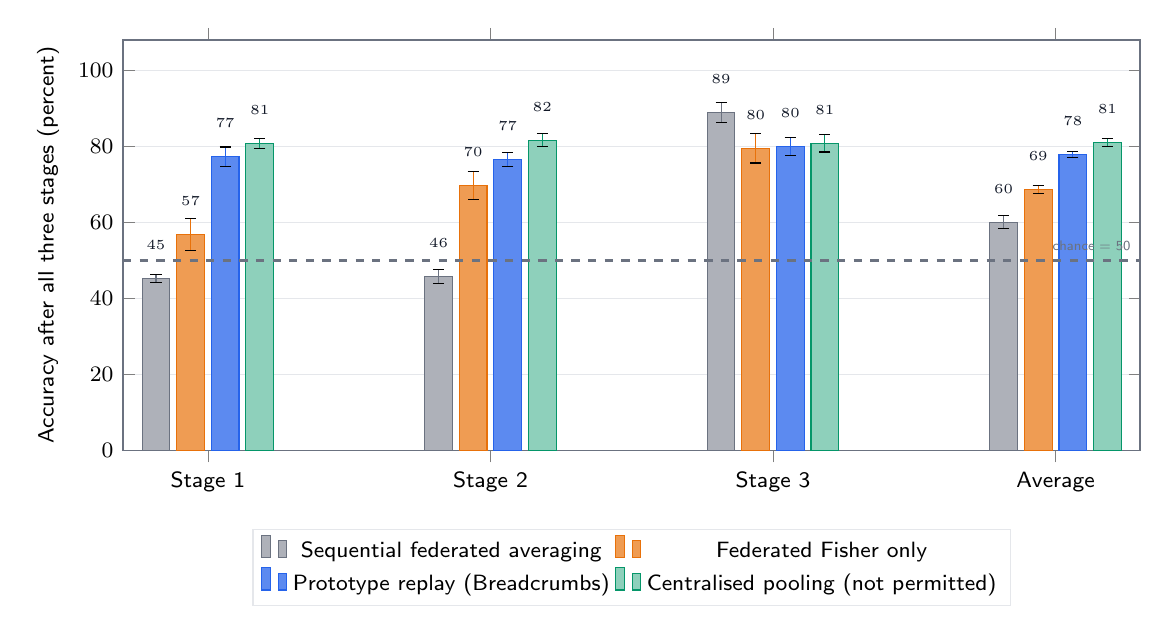
\begin{tikzpicture}
\begin{axis}[
  width=14.5cm, height=6.8cm,
  ybar=2.5pt, bar width=10pt,
  font=\sffamily\small,
  ymin=0, ymax=108, ytick={0,20,40,60,80,100},
  ylabel={Accuracy after all three stages (percent)},
  symbolic x coords={Stage 1, Stage 2, Stage 3, Average},
  xtick=data,
  ymajorgrids=true, grid style={tcline,line width=0.5pt},
  axis line style={tcgrey,line width=0.6pt},
  tick label style={font=\sffamily\footnotesize},
  label style={font=\sffamily\footnotesize},
  legend style={font=\sffamily\footnotesize,at={(0.5,-0.19)},anchor=north,
                legend columns=2,draw=tcline},
  nodes near coords, every node near coord/.append style={
      font=\sffamily\tiny,color=tctext,yshift=7pt,
      /pgf/number format/fixed,/pgf/number format/precision=0},
  error bars/y dir=both, error bars/y explicit,
]
\addplot[fill=tcgrey!55,draw=tcgrey] coordinates {
  (Stage 1,45.2) +- (0,1.1) (Stage 2,45.8) +- (0,1.8)
  (Stage 3,88.9) +- (0,2.7) (Average,60.0) +- (0,1.7)};
\addplot[fill=tcorange!70,draw=tcorange] coordinates {
  (Stage 1,56.8) +- (0,4.3) (Stage 2,69.6) +- (0,3.7)
  (Stage 3,79.5) +- (0,3.9) (Average,68.6) +- (0,1.1)};
\addplot[fill=tcblue!75,draw=tcblue] coordinates {
  (Stage 1,77.3) +- (0,2.5) (Stage 2,76.5) +- (0,1.8)
  (Stage 3,79.9) +- (0,2.3) (Average,77.9) +- (0,0.8)};
\addplot[fill=tcgreen!45,draw=tcgreen] coordinates {
  (Stage 1,80.7) +- (0,1.3) (Stage 2,81.6) +- (0,1.7)
  (Stage 3,80.8) +- (0,2.3) (Average,81.0) +- (0,1.0)};
\draw[tcgrey,dashed,line width=0.9pt]
  ({rel axis cs:0,0}|-{axis cs:Stage 1,50}) -- ({rel axis cs:1,0}|-{axis cs:Stage 1,50});
\node[font=\sffamily\tiny,text=tcgrey,anchor=south east]
  at ({rel axis cs:1,0}|-{axis cs:Stage 1,50}) {chance = 50};
\legend{Sequential federated averaging, Federated Fisher only,
        Prototype replay (Breadcrumbs), Centralised pooling (not permitted)}
\end{axis}
\end{tikzpicture}
\caption{Accuracy on each stage measured after all three stages of training are
complete. The dashed line is chance, 50 percent, because each stage's test set
has two categories. Error bars show one standard deviation over five random
seeds. Sequential federated averaging scores highest on the most recent stage,
88.9 percent, while falling to about 45 percent, below chance, on both earlier
stages. Prototype replay ends 3.1 points below the centralised ceiling that
pooling raw data would give. Simulation on synthetic data, not a deployment
measurement.}
\label{fig:results}
\end{figure}

The pattern for the baseline is the one the continual learning literature
predicts \citep{delange2022survey}. Plain sequential training is excellent at
whatever it learned last and worse than guessing on anything earlier.

\subsection{The mechanism we removed}
\label{sec:removed}

An earlier draft proposed a hybrid: the Fisher penalty and replay together. We
had not run the ablation. When we did, the result went against us. Replay alone
scores 77.9; adding the penalty moves it to 74.0. The penalty buys 1.1 points of
forgetting and costs 3.9 points of accuracy, and 9.2 on the newest stage, at
every difficulty setting we tested.

So we removed it. This reverses a claim we would otherwise have made. We had
written that giving up accuracy on the newest task was the stability and
plasticity trade-off. It was not. It was one of our own components, and deleting
it recovered most of the loss. Breadcrumbs has two mechanisms, not three, and
privacy-preserving replay does the work.

\subsection{How we set the difficulty}
\label{sec:difficulty}

The simulation has a parameter controlling how far apart the four document
categories sit in feature space, which sets how hard detection is. We used 0.50.
Table~\ref{tab:sweep} repeats the whole comparison across a wide range.

Two things in that table are uncomfortable and we would rather present them than
have them found. First, 0.50 is close to the setting that \emph{maximises} the
baseline's forgetting, the 42.0 quoted in our summary; a harder or easier
problem makes the headline gap smaller. Second, from about 1.00 upward the
problem largely disappears on its own, with plain federated averaging reaching
86.1 and only 19.1 forgetting. If real document categories are that well
separated, our mechanism is not needed, and we would rather say so than discover
it in a pilot. What does hold across the whole range is the ordering: replay has
the highest average accuracy of the three federated methods at every setting.

\begin{table}[htbp]
\centering
\caption{The same comparison across seven difficulty settings. Each cell is
average accuracy over the three stages, then forgetting, both in percent and
averaged over five seeds. Higher accuracy is better, lower forgetting is better.
Chance accuracy is 50.0 throughout. The report's main results use the 0.50 row.
Simulation on synthetic data.}
\label{tab:sweep}
\small
\begin{tabular}{@{}c ccccc@{}}
\toprule
\textbf{Separation} & \textbf{Sequential} & \textbf{Fisher} &
\textbf{Prototype} & \textbf{Fisher $+$ replay} & \textbf{Centralised} \\
\textbf{setting} & \textbf{FedAvg} & \textbf{only} & \textbf{replay} &
\textbf{(removed)} & \textbf{pooling} \\
 & ACC / FGT & ACC / FGT & ACC / FGT & ACC / FGT & ACC / FGT \\
\midrule
0.30          & 50.1 / 36.5 & 46.8 / 36.2 & \textbf{57.0} / 13.5 & 56.2 / 11.0 & \textit{59.4} / 0.0 \\
0.40          & 55.1 / 40.1 & 58.2 / 29.7 & \textbf{68.2} / 10.6 & 65.3 / \ \ 9.0 & \textit{70.7} / 0.0 \\
\textbf{0.50} & 60.0 / 42.0 & 68.6 / 22.2 & \textbf{77.9} / \ \ 7.6 & 74.0 / \ \ 6.5 & \textit{81.0} / 0.0 \\
0.60          & 64.6 / 41.3 & 77.4 / 15.9 & \textbf{85.5} / \ \ 5.0 & 81.1 / \ \ 4.3 & \textit{88.3} / 0.0 \\
0.80          & 76.0 / 31.2 & 88.7 / \ \ 8.3 & \textbf{93.9} / \ \ 2.2 & 90.7 / \ \ 2.2 & \textit{95.7} / 0.0 \\
1.00          & 86.1 / 19.1 & 94.8 / \ \ 4.2 & \textbf{97.6} / \ \ 0.8 & 95.8 / \ \ 0.7 & \textit{98.3} / 0.0 \\
1.50          & 97.3 / \ \ 3.9 & 99.4 / \ \ 0.5 & \textbf{99.8} / \ \ 0.1 & 99.2 / $-$0.1 & \textit{99.9} / 0.0 \\
\bottomrule
\end{tabular}
\end{table}

\subsection{A test our own benchmark fails}
\label{sec:probe}

We then asked a harder question of ourselves. Our memory bank is a set of
cluster centres, variances and counts. If that summary describes the data well
enough, someone could skip the federated training entirely, generate synthetic
records from the summary, and train one model centrally. If that worked as well
as our system, then our result would be telling us about the synthetic data
rather than about the method.

We ran it. A model trained only on synthetic records from the memory bank, with
no federated training at all, reaches 77.4 against our 77.9. We then rebuilt the
generator to make features correlated, skewed and heavy-tailed, so a
cluster-and-variance summary is no longer sufficient, and re-ran: 78.1 against
our 79.0. The gap did not open.

We report this because it is the most serious weakness in our evaluation. Where
document categories differ mainly in their average feature values, a compact
summary of those averages carries most of the signal. Any method built on such
summaries then looks good for a reason that has nothing to do with the method.
Our benchmark cannot separate ``prototype replay works'' from ``this data is
easy to summarise''.

Two things follow. The first is that the learning claim in this report should be
read as a mechanism that behaves as designed on synthetic data, and not as
evidence of accuracy on real documents. Settling it requires real factory
records, which is the first thing a pilot produces. The second cuts the other
way. If these summaries are informative enough to train a usable model on their
own, then they leak more than we assumed. That makes the privacy work in
Section~\ref{sec:novel} more urgent, not less.

\subsection{Answering it, partly, on row-level documents}
\label{sec:corpus}

The objection above is specific enough to test, so we tested it. The simulation
behind Figure~\ref{fig:results} runs on Gaussian clusters. Those classes differ
mainly in their average values, which is the easiest possible shape for a summary
of means and variances to capture. So we rebuilt the evaluation on documents
instead. The corpus holds 19{,}980 synthetic compliance records across five record
types, six sites and nine anomaly kinds. They are filed the way a factory really
files them, with four different date formats, numbers stored as text, mixed
capitalisation, and a messiness rate that differs from site to site.

This is not a second sample from the same distribution. The six sites are the
federated clients, and each one gets an uneven share of the anomaly kinds drawn
from a Dirichlet($\alpha{=}0.6$) mixture. The three violation waves are the
continual stages, so by the time wave~3 arrives, wave~1's data is gone. The
detector reads features taken from domain rules: whether stated totals add up,
whether check digits are valid, whether dates run in the right order, and how
leading digits are distributed. None of that can be rebuilt from a summary of
class means, which is what the objection asked for.

Figure~\ref{fig:corpus} and Table~\ref{tab:corpus} give the result. It agrees
with Figure~\ref{fig:results} in direction, and the effect is smaller. Prototype
replay gains 6.6 points of average balanced accuracy over sequential federated
averaging here, against 17.9 points in the simpler simulation. Forgetting halves,
from 16.8 to 8.5. Under sequential averaging, wave~1 falls to exactly chance on
every seed, which is total forgetting, and replay recovers 17.8 points of it. A
smaller effect on harder data is what we expected. A larger one would have made
us suspicious.

\begin{figure}[htbp]
\centering
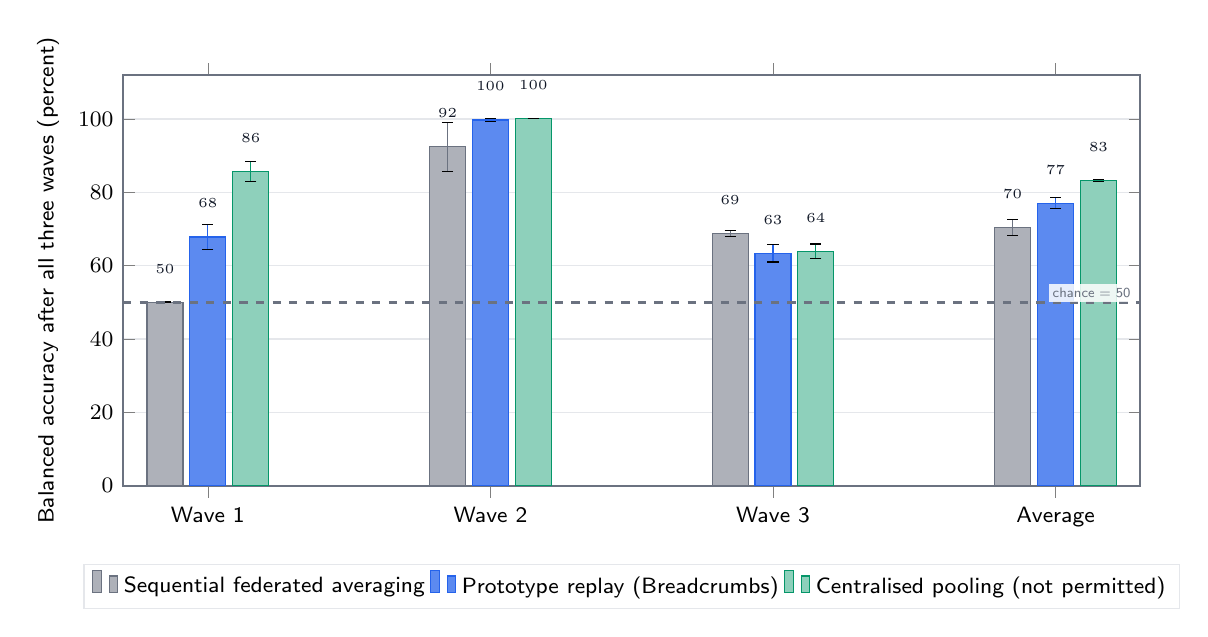
\begin{tikzpicture}
\begin{axis}[
  width=14.5cm, height=6.8cm,
  ybar=2.5pt, bar width=13pt,
  font=\sffamily\small,
  ymin=0, ymax=112, ytick={0,20,40,60,80,100},
  ylabel={Balanced accuracy after all three waves (percent)},
  symbolic x coords={Wave 1, Wave 2, Wave 3, Average},
  xtick=data,
  ymajorgrids=true, grid style={tcline,line width=0.5pt},
  axis line style={tcgrey,line width=0.6pt},
  tick label style={font=\sffamily\footnotesize},
  label style={font=\sffamily\footnotesize},
  legend style={font=\sffamily\footnotesize,at={(0.5,-0.19)},anchor=north,
                legend columns=3,draw=tcline},
  nodes near coords, every node near coord/.append style={
      font=\sffamily\tiny,color=tctext,yshift=7pt,
      /pgf/number format/fixed,/pgf/number format/precision=0},
  error bars/y dir=both, error bars/y explicit,
]
\addplot[fill=tcgrey!55,draw=tcgrey] coordinates {
  (Wave 1,50.0) +- (0,0.1) (Wave 2,92.4) +- (0,6.7)
  (Wave 3,68.8) +- (0,0.9) (Average,70.4) +- (0,2.1)};
\addplot[fill=tcblue!75,draw=tcblue] coordinates {
  (Wave 1,67.8) +- (0,3.4) (Wave 2,99.7) +- (0,0.5)
  (Wave 3,63.4) +- (0,2.4) (Average,77.0) +- (0,1.5)};
\addplot[fill=tcgreen!45,draw=tcgreen] coordinates {
  (Wave 1,85.7) +- (0,2.7) (Wave 2,100.0) +- (0,0.0)
  (Wave 3,63.9) +- (0,2.0) (Average,83.2) +- (0,0.3)};
\draw[tcgrey,dashed,line width=0.9pt]
  ({rel axis cs:0,0}|-{axis cs:Wave 1,50}) -- ({rel axis cs:1,0}|-{axis cs:Wave 1,50});
\node[font=\sffamily\tiny,text=tcgrey,anchor=south east,
      fill=white,fill opacity=0.85,text opacity=1,inner sep=1.5pt]
  at ({rel axis cs:0.995,0}|-{axis cs:Wave 1,50}) {chance = 50};
\legend{Sequential federated averaging, Prototype replay (Breadcrumbs),
        Centralised pooling (not permitted)}
\end{axis}
\end{tikzpicture}
\caption{Federated continual learning on the document corpus, five seeds. Six
sites are the federated clients; the three violation waves are the continual
stages. Measured at the 10\% false-positive budget of
Table~\ref{tab:corpus_operating}.}
\label{fig:corpus}
\end{figure}

\textbf{The operating point is a decision, and we had been avoiding it.} Our
first version of this experiment picked a class with a four-way $\arg\max$. That
has no threshold to set. It flagged 39.1\% of clean documents, which means two in
every five honest records would go to an auditor, and the number moved between
9\% and 43\% when nothing changed but the random seed. That is not a property of
the model. It is what happens when nobody chooses. We now score each document by
$P(\text{anomalous})$ and compare it against a threshold picked on a held-out
slice of the \emph{training} data. The false-positive rate becomes a number the
consortium sets. Table~\ref{tab:corpus_operating} gives the curve. ROC-AUC is
$0.894\,\pm\,0.004$, and because it does not depend on the threshold, it is the
right number for comparing methods.

\textbf{What this settles, and what it does not.} It answers the objection. The
result holds on data that a summary of means and variances cannot describe, so
``prototype replay works'' can now be told apart from ``this data is easy to
summarise''. It does not make the corpus real. These are still invented documents
with an anomaly rate we chose, and the detector still reads hand-built statistics
rather than raw rows. Table~\ref{tab:corpus_kinds} carries the control that keeps
us honest. A \texttt{cross\_inconsistency} document is internally consistent and
disagrees with a \emph{different} document from the same period, so nothing in a
single document can reveal it. Those documents are flagged less often than clean
ones are. If that row had shown a high detection rate, something in the pipeline
would have been wrong.


\begin{table}[htbp]
\centering
\caption{Federated continual learning on the document corpus, mean and standard
deviation over five seeds. Six sites act as federated clients with a
Dirichlet($\alpha{=}0.6$) partition; the three violation waves are the continual
stages. Balanced accuracy is reported because 4.11\% of the corpus is anomalous
and plain accuracy would reward a detector that finds nothing; chance is 50.0.
Recall is measured as filing a document under the correct wave, not merely
flagging it. Every figure is measured at the 10\% false-positive budget of
Table~\ref{tab:corpus_operating}. Backward transfer is $-25.2\,\pm\,3.5$ for
sequential averaging and $-12.7\,\pm\,2.0$ for prototype replay. Unlike
Table~\ref{tab:results}, these are row-level documents with nine anomaly kinds,
not Gaussian clusters.}
\label{tab:corpus}
\small
\setlength{\tabcolsep}{4.5pt}
\begin{tabular}{@{}l c c c c c@{}}
\toprule
\textbf{Method} & \textbf{Wave 1} & \textbf{Wave 2} & \textbf{Wave 3} &
\textbf{Average} & \textbf{Forgetting} \\
\midrule
Chance & 50.0 & 50.0 & 50.0 & 50.0 & n/a \\
Sequential federated averaging & 50.0\,$\pm$\,0.1 & 92.4\,$\pm$\,6.7 &
  \textbf{68.8\,$\pm$\,0.9} & 70.4\,$\pm$\,2.1 & 16.8\,$\pm$\,2.3 \\
\textbf{Prototype replay (ours)} & \textbf{67.8\,$\pm$\,3.4} &
  \textbf{99.7\,$\pm$\,0.5} & 63.4\,$\pm$\,2.4 & \textbf{77.0\,$\pm$\,1.5} &
  \textbf{8.5\,$\pm$\,1.3} \\
\midrule
\textit{Centralised pooling (not permitted)} & \textit{85.7\,$\pm$\,2.7} &
  \textit{100.0\,$\pm$\,0.0} & \textit{63.9\,$\pm$\,2.0} & \textit{83.2\,$\pm$\,0.3} &
  \textit{n/a} \\
\bottomrule
\end{tabular}
\end{table}

\begin{table}[htbp]
\centering
\caption{Choosing the operating point. A four-way $\arg\max$ has no adjustable
threshold, and the point it happens to land on gave a false-positive rate of
39.1\,$\pm$\,8.0, which is unusable for an auditor and unstable across seeds. Scoring
instead on $P(\text{anomalous})$ against a threshold chosen on a held-out 15\%
split of the \emph{training} shards makes the false-positive rate a quantity the
consortium sets. The benchmarks are never used to choose it. ROC-AUC is
$0.894\,\pm\,0.004$ and does not depend on the threshold at all. Note that the
5\% budget dominates the 10\% one: it scores higher balanced accuracy while
flagging half as many clean documents.}
\label{tab:corpus_operating}
\small
\begin{tabular}{@{}l r r r@{}}
\toprule
\textbf{False-positive budget} & \textbf{Detection} & \textbf{Realised FP} &
\textbf{Balanced} \\
\midrule
1\%  & 67.3\,$\pm$\,1.9 &  1.0\,$\pm$\,0.2 & 83.1\,$\pm$\,1.0 \\
5\%  & 74.4\,$\pm$\,1.8 &  5.1\,$\pm$\,0.5 & \textbf{84.7\,$\pm$\,0.9} \\
10\% & 77.3\,$\pm$\,2.3 & 10.4\,$\pm$\,0.8 & 83.5\,$\pm$\,1.2 \\
\midrule
\textit{$\arg\max$, no threshold (previous)} & \textit{88.7} & \textit{43.2} &
  \textit{72.8} \\
\bottomrule
\end{tabular}
\end{table}

\begin{table}[htbp]
\centering
\caption{Detection by anomaly kind on the held-out cross-wave benchmark, for the
prototype-replay detector after all three waves, at the 10\% budget. Mean and
standard deviation over the same five seeds. The false-positive rate is given in
the same table rather than a footnote, because a per-kind detection rate without
it is not a result: a model that answers ``anomalous'' more often scores better
on every row and is worse at the job. \texttt{cross\_inconsistency} is the
control. Those documents are internally consistent and contradict a
\emph{different} document of the same period, so no single-document feature can
see them, and at 8.3\% they are flagged \emph{less} often than clean documents
are, which is the correct result and the one we would have had to explain away
had it come out otherwise.}
\label{tab:corpus_kinds}
\small
\begin{tabular}{@{}l r r@{}}
\toprule
\textbf{Anomaly kind} & \textbf{Detected} & \textbf{$n$} \\
\midrule
Back-dated signature          & 100.0\,$\pm$\,0.0 &  98 \\
Benford first-digit violation & 100.0\,$\pm$\,0.0 & 145 \\
Certificate / CAS check digit & 100.0\,$\pm$\,0.0 & 125 \\
Arithmetic inconsistency      &  99.2\,$\pm$\,0.4 &  95 \\
Duplicated reference          &  90.4\,$\pm$\,13.5 & 160 \\
Implausible roundness         &  80.0\,$\pm$\,15.5 &  39 \\
Overtime above the ceiling    &  70.9\,$\pm$\,17.6 &  11 \\
Site-relative outlier         &  50.1\,$\pm$\,1.6 & 284 \\
\midrule
\textit{Clean documents (false positives)} & \textit{10.4\,$\pm$\,0.8} & \textit{971} \\
\textit{Cross-document inconsistency (control)} & \textit{8.3\,$\pm$\,5.1} & \textit{70} \\
\bottomrule
\end{tabular}
\end{table}


\section{What is built, and what is not}
\label{sec:proto}

An earlier version of this report proposed a fourteen-week build. Most of it now
exists, and the honest thing is to say precisely which parts, because ``we built
it'' is a claim a judge is entitled to check line by line.

\textbf{What runs.} A permissioned blockchain written in Python: X.509 membership
with RSA-3072 identities, endorsement policies evaluated over distinct
organisations, a Raft-style ordering service, deterministic chaincode, hash-chained
blocks and a versioned world state with multi-version concurrency control. Four
contracts run on it: \texttt{doccustody} for commitments, seals, witnesses and
findings; \texttt{anchor} for the accumulator and the delay beacon;
\texttt{fedmodel} for the Continuity Gate; \texttt{reputation} for contribution
scores. Above them sit the accumulator library, the Merkle disclosure layer, the
federated continual learning plane, a FastAPI backend and a React client. It needs
no Docker and runs on any laptop.

\textbf{What that is not.} It is \emph{Fabric-modelled}, not Fabric. The
architecture follows Hyperledger Fabric's execute--order--validate model and the
chaincodes are also written as real Fabric contracts in \texttt{model/fabric/}
with a \texttt{docker-compose} network, but \textbf{no Fabric peer has ever run
them}. Where a number in this report comes from the Python chain, that is what we
claim, and every performance figure in Section~\ref{sec:performance} is labelled
accordingly. Running the real deployment is the next task and it needs a machine
with Docker and 16 gigabytes.

\textbf{How it is tested.} 273 tests, of which 27 name a specific attacker and
attempt the attack. Two of those attacks succeed and a third is bounded rather
than prevented; all three are reported in Section~\ref{sec:security}. The suite was written the way our own
security audit recommends: for every guarantee the system asserts, a test that
tries to break it. That discipline found two critical flaws during the audit.
Endorsement signatures were verified against a caller-supplied key, and a single
actor could forge every organisation's Continuity Gate evaluation. Either of these
would have made the project's headline guarantee false while the demonstration
appeared to work perfectly.

\textbf{The data.} A generator produces invented documents across five types with
planted, labelled anomalies: arithmetic that does not add up, certificate
identifiers failing a checksum, overtime beyond the legal ceiling, back-dated
entries, and values far from a site's own normal. Nothing in it is real, the
anomaly rate is chosen rather than observed, and no claim about the industry
follows from it. A second-generation corpus, specified in the supplementary
material, adds row-level records and, more importantly, a labelled
\emph{adversary trace} of attempted tampering, withholding, back-dated seals and
witness collusion, without which the ledger's guarantees can be asserted but not
scored.

\textbf{The demonstration} performs a full cycle: commits documents, seals a
reporting period, discloses a subset and watches the completeness check catch it,
folds an epoch into the accumulator, and submits two model candidates, one that
improves everything and is promoted, one that damages an earlier task and is
rejected on-chain. That rejection, and the withheld-record refusal, are the two
moments worth showing.

\begin{table}[htbp]
\centering
\caption{What exists and what does not, as of this report.}
\label{tab:plan}
\small
\begin{tabularx}{\textwidth}{@{}l l Y@{}}
\toprule
\textbf{Component} & \textbf{State} & \textbf{Note} \\
\midrule
Permissioned ledger, RSA identities & Built & Fabric-modelled, in Python; runs on any laptop \\
\texttt{doccustody}: commitments, grants & Built & Merkle selective disclosure over HTTP \\
Period seals and completeness & Built & The claim in Section~\ref{sec:seals} \\
Attesting witnesses, commit--reveal seed & Built & Adoption is a governed act, off until a round closes \\
Accumulator, absence and batching proofs & Built & With the trusted-dealer ceremony recorded on-chain \\
Delay beacon and epoch digests & Built & Fork detection across members \\
Continuity Gate & Built & Every branch of Algorithm~\ref{alg:gate} tested \\
Federated continual learning & Built & Prototype replay, clipping, noise, trimmed mean \\
Backend API and client & Built & Capability-table authorization \\
Real Hyperledger Fabric deployment & \textbf{Written, never run} & Needs Docker and 16\,GB \\
Orderer block signatures & \textbf{Not built} & Audit gap, ordinary work \\
Client-side proposal signatures & \textbf{Not built} & Audit gap, ordinary work \\
Secure aggregation & \textbf{Not built} & Conflicts with contribution scoring, disclosed \\
Row-level detector, second corpus & \textbf{Specified} & Supplementary material \\
Pilot with real documents & \textbf{Not started} & The only thing that settles the learning claim \\
\bottomrule
\end{tabularx}
\end{table}

The whole prototype runs on one laptop with 16 gigabytes of memory. A production
peer node for one factory fits comfortably on a small cloud instance, which
listed at roughly 60 to 120 US dollars per month with major providers in 2026.
That figure is a published list price, not a measured operating cost.

% =============================================================================
\section{Impact and the Sustainable Development Goals}

We would rather claim less and be able to measure it than claim more. Every row
of Table~\ref{tab:sdg} names a number the pilot can actually produce.

\begin{table}[htbp]
\centering
\caption{How Breadcrumbs connects to the Sustainable Development Goals
\citep{un2015sdg}, and what we would measure during a pilot to show it.}
\label{tab:sdg}
\small
\begin{tabularx}{\textwidth}{@{}l Y Y@{}}
\toprule
\textbf{Goal} & \textbf{How the system contributes} & \textbf{What we measure} \\
\midrule
\textbf{8} Decent work &
Wage registers, overtime logs and grievance records become tamper-evident, so a
worker's claim can be checked against a record that could not be rewritten
afterwards. &
Share of payroll periods committed within 48 hours; number of grievance records
with verifiable timestamps. \\
\textbf{5} Gender equality &
Women hold more than half the jobs in this sector, and wage and grievance
records are the documents that most affect them. Verifiable records make
under-payment harder to conceal. &
Share of committed wage records covering female workers; grievance resolution
time before and after. \\
\textbf{9} Industry and innovation &
Gives small suppliers a way to prove compliance digitally without buying a
separate system for every buyer. &
Number of factories active; documents committed per factory per month. \\
\textbf{12} Responsible production &
Chemical inventories and environmental logs become auditable evidence that can
feed a Digital Product Passport instead of a separate declaration. &
Share of chemical records committed; number of passport claims backed by a
verified hash. \\
\textbf{16} Strong institutions &
Audit findings and access grants are recorded permanently, which reduces the
room for an inspection outcome to be quietly negotiated. &
Number of independently verified disclosures; count of Continuity Gate
rejections recorded. \\
\textbf{17} Partnerships &
A shared consortium across factories, buyers, auditors and a regulator observer,
with no single owner. &
Number of participating organisation types; cross-border verifications served. \\
\bottomrule
\end{tabularx}
\end{table}

There is also an effect we cannot measure but should state. Bangladesh's garment
sector has spent a decade being told to prove itself, largely on terms set
elsewhere. A verification system designed and operated in Bangladesh changes who
holds the evidence. The National Blockchain Strategy identified this kind of
application as a national priority \citep{ictd2020blockchain}, and the
underlying argument for blockchain in supply chains is well established in the
research literature \citep{saberi2019blockchain,kshetri2018blockchain}.

% =============================================================================
\section{Who pays, and how this gets adopted}

The hardest question for any consortium system is why the third participant
joins when the network effect needs the thirtieth. Breadcrumbs has to be useful
to a single factory on day one, before any consortium exists.

It is. Plane A works alone: one factory, one node, no partners, committing its
documents and proving to any buyer that they are authentic and unchanged. That
is a complete product with no dependency on anyone else. The shared detector in
Plane B becomes possible once several factories join. It is the reason to stay,
not the reason to start.

Factories pay an annual subscription by size. Table~\ref{tab:money} sets out an
illustrative model. Every figure in it is an assumption we have stated, not a
measurement, and the revenue column is simply the multiplication of the two
columns before it.

\begin{table}[htbp]
\centering
\caption{Illustrative revenue model. All figures are assumptions for planning,
not measured results. Buyers and auditors pay separately for verification
access, which is not counted here.}
\label{tab:money}
\small
\begin{tabular}{@{}l c c c l@{}}
\toprule
\textbf{Year} & \textbf{Factories} & \textbf{Average fee (USD)} &
\textbf{Revenue (USD)} & \textbf{Stage} \\
\midrule
1 & 6   & 0     & 0       & Free pilot, grant funded \\
2 & 60  & 2{,}400 & 144{,}000 & Paid pilot with two buyer partners \\
3 & 300 & 3{,}000 & 900{,}000 & BGMEA-level rollout \\
\bottomrule
\end{tabular}
\end{table}

Against that, the saving to a factory is the part we can argue but not yet
prove, and the arithmetic does not currently close. Two avoided audits a year at
a starting price near 800 US dollars is 1{,}600 dollars, against a year-two fee
of 2{,}400. That covers about two thirds of the fee, not all of it. We could
close the gap by quoting a higher audit price. Multi-pillar audits at a
2{,}000-worker site cost considerably more than the entry-level figure we used.
But we do not have a sourced number for that, and will not invent one.

So we state it as it is. On defensible numbers, avoided audits cover most of the
subscription and the rest must come from less staff time assembling evidence,
fewer delayed shipments, and better terms from buyers who can verify claims
cheaply. Those are plausible and unmeasured.

The binding constraint is not the arithmetic anyway. Avoiding an audit requires a
\emph{buyer} to accept cryptographic evidence instead of a visit, and no buyer
has agreed to that. Under the coming liability a buyer's first instinct will be
to audit more, not less. Our honest expectation is that Breadcrumbs first makes
audits cheaper and better targeted rather than removing them, and that
replacement becomes possible only after a large buyer has run it alongside its
existing process long enough to trust it.

Adoption runs in three steps. First, six factories and one willing buyer, which
is small enough to run without institutional permission. Second, an approach to
BGMEA to position Breadcrumbs as the internal-records layer beneath the Digital
Product Passport work it has already committed to
\citep{bgmea2025digiprod,bgmea2026aware}, rather than as a competing platform.
Third, the system crosses borders along a route that already exists. The buyers
placing orders in Bangladesh place them in Vietnam, India, Cambodia and Turkey
too, under the same European rules and the same liability. A buyer requiring
verifiable records from Bangladeshi suppliers has reason to require them from
all suppliers, because partial coverage does not reduce its legal exposure. That
makes the buyer, not us, the party who carries the system into the next country.
Bangladesh gains from moving first: the country that already has the
infrastructure becomes the easy supplier to keep, exactly when tariff
preferences stop making it the cheap one. The same architecture then moves to
any sector with many mutually distrustful organisations, confidential internal
records, and rules that keep changing. Pharmaceuticals, food processing and
non-bank financial institutions all qualify.

% =============================================================================
\section{Hard questions we expect, and our answers}
\label{sec:hardquestions}

\textbf{``A blockchain cannot tell whether the document was true in the first
place. You have built a perfect record of a possible lie.''}
Correct, and it is the most serious limitation of every provenance system ever
built, including ours. We do not claim to verify truth. We claim to remove the
ability to change a record afterwards, which is narrower and still valuable.
Today a factory that finds a problem in March can produce a clean March file in
June. Under Breadcrumbs it cannot, because the June file will not match the
March commitment. Three measures narrow the remaining gap. Capture at source
commits records automatically from the payroll or machine system, rather than
having them typed in later. Cross-checking compares a wage total against
production output and electricity readings committed by different systems, which
are hard to falsify together. And the detector itself is trained on exactly this
kind of inconsistency. What is left is a first-mile problem we should be judged on
honestly rather than pretend to have solved.

\textbf{``Why would a factory adopt a system that makes its own violations
undeniable?''}
Because a compliant factory gets no credit today: its records look exactly like
a non-compliant factory's. Verifiability is an advantage for the good operator
and a threat only to the bad one. Adoption is also partial by design: a factory
chooses which document types to commit, and buyers widen that over time.

\textbf{``Why not a database with signed audit logs and a public transparency
log?''}
That design is genuinely close and we considered it. It fails on one point:
somebody must operate it, and whoever does can refuse to serve a proof, reorder
events, or lose an inconvenient record. The parties here have concrete reasons
to distrust each other, as Section~\ref{sec:whychain} sets out. A permissioned ledger with an
endorsement policy removes that single point of control. If a neutral,
well-funded, permanent operator existed and all parties accepted it, a database
would be the better engineering choice, and we would say so.

\textbf{``Federated learning leaks. Model updates can be inverted to recover
training data.''}
Yes, and we cite that work rather than avoid it
\citep{zhu2019dlg,geiping2020inverting}. Federated learning is not private on
its own, and we will not list defences we have not committed to. In the first
deployment the protections are clipped updates, added noise, and locally
engineered features so raw text never enters the model. We do \emph{not} run
secure aggregation, because it cannot coexist with the robust averaging and
contribution scoring we need on day one (Section~\ref{sec:planeb}). That is weaker than the
literature's best, it is in our limitations, and it is the first thing we would
strengthen.

\textbf{``What stops a factory poisoning the shared model, or free-riding?''}
Poisoning is countered by trimmed-mean aggregation, which tolerates a minority
of dishonest participants \citep{yin2018byzantine,bagdasaryan2020backdoor}, and
by the Continuity Gate rejecting any candidate that damages committed
benchmarks. Free-riding is countered by the reputation chaincode: access to the
current model is conditional on a recorded contribution history.

\textbf{``Personal data on an immutable ledger conflicts with deletion
rights.''}
Which is why no personal data goes on the ledger. Only salted hashes are
committed, and deleting the off-chain record leaves the hash a meaningless
string with nothing to compare against. That satisfies erasure while leaving the
audit trail intact.

\textbf{``BGMEA already signed two blockchain agreements. Why do you exist?''}
Because those agreements cover Digital Product Passports, which describe
products and materials. Neither covers a factory's internal operating records,
and neither involves shared learning. We are complementary by design. A passport
claim is only worth what the internal record behind it is worth, and that record
is what we make provable.

\textbf{``What if a factory loses its signing key?''}
Keys are issued by the Fabric membership service and held in the factory's own
hardware security module, with recovery requiring approval from a threshold of
consortium members. Historical commitments stay valid because they were signed
by a key valid at the time. Rotation and revocation are ordinary transactions,
not exceptional events.

\textbf{``What is the throughput, and is it enough?''}
A factory produces hundreds of committed documents a month. Even a thousand
factories sits far below what Hyperledger Fabric sustains
\citep{androulaki2018fabric,dinh2018untangling}. Being unambitious about
throughput is a strength: this workload does not stress the technology, so
performance is not where the risk sits.

\textbf{``IBM already holds a patent on a smart contract that checks a model
against a threshold. What is left of your novelty?''}
Less than our first draft claimed, and we corrected it rather than defend it.
US 11{,}157{,}833 covers checking a submitted model against a withheld test set
and a performance threshold \citep{calmon2021patent}, and LiFeChain already puts
federated lifelong learning on a blockchain \citep{chen2025lifechain}. What
remains is narrower: a promotion rule that looks \emph{backward} across a set of
per-task benchmarks committed in advance, enforced by a threshold of independent
organisations rather than by one owner. The patent is a commercial fact as well
as an academic one, and any team taking this to market needs legal advice on it.
We would rather raise that than have an investor find it in diligence.

\textbf{``What if the consortium dissolves?''}
Every factory keeps its own documents and its own copy of the commitments.
Hashes stay verifiable against any preserved copy of the ledger, and the formats
are open. A participant that leaves loses the shared detector, not its evidence.

A fuller record of the hostile review this system was put through is in
\texttt{AUDIT.md} in the repository: five serious findings, two of which made the
project's headline guarantee false while the demonstration appeared to work
perfectly. Both were in signature verification, both looked correct on a casual
read, and neither would have been caught by any test that only exercises the
happy path.

% =============================================================================
\section{What we cannot do yet}
\label{sec:limits}

Collected in one place, so nobody has to find them scattered through the report.

\begin{enumerate}[leftmargin=1.4em,itemsep=0.15em]
\item \textbf{Two attacks in our own suite succeed, and a third is bounded
rather than prevented} (Section~\ref{sec:security}). A colluding assigned witness
is not stopped, and is bounded in cost rather than prevented: falsification now
requires two organisations, both named, and the witness loses more than it earned.
The holder of the modulus's factorisation can forge a membership witness against
the accumulator alone, and is defeated by the other two verification checks but
not by the accumulator itself. The third, a model poisoned just inside the gate's
tolerance, is promoted for one round as it should be, but repeating it is caught
by the $\sigma$ drift bound.
\item The Continuity Gate bounds regression per round at $\tau$ and cumulatively
at $\sigma$ against each task's best-ever score. An adversary willing to lose
slightly less than the tolerance every round is therefore capped at $\sigma$ of
total damage rather than unbounded, but $\sigma$ is still available to it, and
the right value is a consortium's judgement rather than something we can derive.
\item Period seals defeat withholding at disclosure. They do not compel a factory
to commit a record in the first place, so a document kept entirely off the ledger
leaves a seal that is internally consistent and silent.
\item The accumulator modulus comes from a \emph{trusted-dealer} ceremony with
member entropy and a stored transcript, not from distributed generation. A
dishonest dealer retains a trapdoor. The design is arranged so that this cannot
rewrite history, which is a weaker statement than the trapdoor not existing.
\item RSA-3072 is disallowed after 2035 under NIST IR 8547 \citep{nist2024ir8547}. Signatures and
identities carry a suite identifier and can be re-anchored under a successor, but
\textbf{the accumulator cannot}: no post-quantum construction with constant-size
witnesses is known. The hash chain and the Merkle commitments are the
quantum-durable part of this system; the accumulator is an accelerator with a
horizon.
\item Blocks are not signed by the ordering service and the submitting client does
not sign its own proposal. Both are ordinary work, both are open.
\item The witness rule is a consortium policy that must be adopted through a
commit--reveal round. Before adoption the contract does not require
counter-signatures, and any interface must show that the rule is not in force
rather than imply a guarantee that is switched off.
\item All measurements are from a single process against one SQLite file with no
network between peers, so they are a floor on cost rather than a prediction. The
real Hyperledger Fabric deployment in \texttt{model/fabric/} has never been run.
\item Our benchmark cannot validate the learning claim
(Section~\ref{sec:ablation}). A model trained only on synthetic records from the
memory bank reaches almost the same accuracy as the full method, so the result may
be telling us about the data rather than about the mechanism. Only real documents
settle it.
\item We removed the Fisher penalty after measuring it, so the method changed
during the work; and we chose the difficulty setting, which sits near the value
that makes the baseline look worst.
\item Our added noise is not differential privacy: no sensitivity bound, no
budget, and the released variances and counts are unnoised.
\item Secure aggregation, robust averaging and contribution scoring cannot all
three hold, and the first deployment gives up secure aggregation.
\item Infrastructure is costed from list prices, and the audit saving depends on
buyers accepting cryptographic evidence, which none has yet agreed to do.
\end{enumerate}

Future work follows directly. The immediate step is a pilot with real documents
under a confidentiality agreement, which turns every simulated number in this
report into a measured one. Beyond that, we want to test whether the memory bank
can be reduced further using generative replay \citep{shin2017dgr}, and whether
the Continuity Gate threshold can be set automatically from the consortium's own
error costs rather than negotiated.

% =============================================================================
\section{Conclusion}

Bangladesh's garment industry is asked to prove things about itself constantly
and currently cannot, because its records are not provable and its evidence
cannot be pooled. Breadcrumbs addresses both halves: a permissioned ledger makes
a company's own documents verifiable without publishing them, and federated
learning turns thousands of isolated archives into one shared detector without
moving a file.

The part we consider new is narrower than either of those and we would rather
state it narrowly than have it trimmed for us. Every provenance system on the
market proves that a document is genuine. None proves that the set you were shown
is the whole set, and the fraud that actually happens is not a forged register
but a second one, and a decision about which to disclose. A sealed reporting
period turns that decision into an arithmetic contradiction: the four registers a
factory does hand over all verify perfectly, and the count and the root say that
a fifth existed. Around that sit three mechanisms sharing one RSA group:
constant-size verifier state, proofs of absence, constant-time epoch checking, and
a delay function that stops history being manufactured faster than it can be
lived. And beside it sits an independent counter-signatory who is assigned rather
than chosen and who has something to lose.

We have tried to be equally clear about what is not true. Two attacks in our own
test suite succeed and are reported as successes, and a third is bounded rather
than prevented. The Continuity Gate bounds regression both per round and
cumulatively, but a determined participant can still spend that budget. Sealing
defeats withholding, not never-recording. The witness converts unilateral falsification into two-party
collusion rather than preventing it. The accumulator modulus has a dealer, and the
design is arranged so that a trapdoor cannot rewrite history, which is a weaker
statement than the trapdoor not existing. RSA-3072 is disallowed after 2035, and
the accumulator, unlike the signatures, has no post-quantum successor to migrate
to. The learning results are on invented data, and our own probe cannot separate
``the mechanism works'' from ``this data is easy to summarise''.

What we can say is that the system runs, that its guarantees have tests that try
to break them, that every performance number in this report was produced by a
benchmark rather than typed. Two claims we would defend hardest are that a
withheld record is caught by arithmetic, and that no single participant can
promote a model. Each is demonstrated by a test that fails against the previous version
of the code. That combination, rather than any individual mechanism, is what we
would ask to be judged on.

% =============================================================================
\small
\begingroup
% Long bibliography URLs sometimes leave deliberately loose lines. They do not
% protrude into the margin, so do not report them as bad boxes.
\hbadness=10000
\bibliographystyle{plainnat}
\bibliography{ref}
\endgroup

\end{document}
